%!TEX root = ../hall.tex
% Тип документа
\documentclass[a4paper,12pt]{extarticle}

% Шрифты, кодировки, символьные таблицы, переносы
% \usepackage{cmap}
% \usepackage[T2A]{fontenc}
\usepackage[utf8]{inputenc}
\usepackage[russian]{babel}
% Это пакет -- хитрый пакет, он нужен но не нужен
\usepackage[mode=buildnew]{standalone}

\usepackage
	{
		% Дополнения Американского математического общества (AMS)
		amssymb,
		amsfonts,
		amsmath,
		amsthm,
		% Пакет для физических текстов
		physics,
		% misccorr,
		% 
		% Графики и рисунки
		wrapfig,
		graphicx,
		subcaption,
		float,
		tikz,
		tikz-3dplot,
		caption,
		csvsimple,
		color,
		booktabs,
		geometry,
		% 
		% Таблицы, списки
		makecell,
		multirow,
		indentfirst,
		%
		% Интегралы и прочие обозначения
		ulem,
		esint,
		esdiff,
		% 
		% Колонтитулы
		fancyhdr,
	}  
\usepackage{pgfplots,pgfplotstable,booktabs,colortbl}
\usepackage{xcolor}
\usepackage{hyperref}
\usepackage{pythontex}
 % Цвета для гиперссылок
\definecolor{linkcolor}{HTML}{000000} % цвет ссылок
\definecolor{urlcolor}{HTML}{799B03} % цвет гиперссылок
 
\hypersetup{pdfstartview=FitH,linkcolor=linkcolor,urlcolor=urlcolor, colorlinks=true}
\hypersetup{pageanchor=false}
% Увеличенный межстрочный интервал, французские пробелы
\linespread{1.3} 
\frenchspacing 

 
% \usetikzlibrary
% 	{
% 		decorations.pathreplacing,
% 		decorations.pathmorphing,
% 		patterns,
% 		calc,
% 		scopes,
% 		arrows,
% 		fadings,
% 		through,
% 		shapes.misc,
% 		arrows.meta,
% 		3d,
% 		quotes,
% 		angles,
% 		babel
% 	}
% Среднее <#1>
\newcommand{\mean}[1]{\langle#1\rangle}

\begin{pycode}
##
def frexp10(decimal):
	parts = ('%e' % decimal).split('e')
	return float(parts[0]), int(parts[1])
##
\end{pycode}
% Функция для тех, кто использует pythontex. Представляет любое вещественное число в стандартном виде.
\newcommand{\frexp}[1]{
		\pyc{#10=frexp10(#1)} 
			\py{ round(#10[0],2)} 
				\cdot 10^{\py{#10[1]}} }

% const прямым шрифтом
\newcommand\ct[1]{\text{\rmfamily\upshape #1}}
\newcommand*{\const}{\ct{const}}
\usepackage{array}
\usepackage{pstool}

\geometry		
	{
		left			=	2cm,
		right 			=	2cm,
		top 			=	2.5cm,
		bottom 			=	2.5cm,
		bindingoffset	=	0cm
	}

%%%%%%%%%%%%%%%%%%%%%%%%%%%%%%%%%%%%%%%%%%%%%%%%%%%%%%%%%%%%%%%%%%%%%%%%%%%%%%%
	%применим колонтитул к стилю страницы
\pagestyle{fancy} 
	%очистим "шапку" страницы
% \fancyhead{} 
	%слева сверху на четных и справа на нечетных
\fancyhead[R]{}%\labauthors 
	%справа сверху на четных и слева на нечетных
% \fancyhead[L]{Отчёт по лабораторной работе №\labnumber}
\fancyhead[L]{\labtheme} 
	%очистим "подвал" страницы
% \fancyfoot{} 
	% номер страницы в нижнем колинтуле в центре
\fancyfoot[C]{\thepage} 

%%%%%%%%%%%%%%%%%%%%%%%%%%%%%%%%%%%%%%%%%%%%%%%%%%%%%%%%%%%%%%%%%%%%%%%%%%%%%%%

\renewcommand{\contentsname}{Оглавление}
\usepackage{tocloft}
\usepackage{secdot}
\sectiondot{subsection}
\usepackage{gensymb}
\usepackage{textcomp}
\usepackage{mathrsfs}
\begin{document}
\def\labauthors{Карусевич А.А, Понур К.А.}
\def\labgroup{430}
\def\department{Кафедра электроники и квантовой физики}
\def\labnumber{1}
\def\labtheme{Движение носителей заряда в электрических и магнитных полях}

\renewcommand{\phi}{\varphi}

\def\E{\mathscr{E}_H}
\def\Rdim{\,\frac{\text{м}^3}{\text{А} \cdot \text{с}}}
\begin{titlepage}

\begin{center}

{\small\textsc{Нижегородский государственный университет имени Н.\,И. Лобачевского}}
\vskip 1pt \hrule \vskip 3pt
{\small\textsc{Радиофизический факультет. Кафедра Радиотехники.}}

\vfill

{\Large Отчет по лабораторной работе №\labnumber\vskip 12pt\bfseries \labtheme}
	
\end{center}

\vfill
	
\begin{flushright}
	{Выполнили студенты \labgroup\ группы\\ \labauthors}%\vskip 12pt Принял:\\ Менсов С.\,Н.}
\end{flushright}
	
\vfill
	
\begin{center}
	Нижний Новгород, \the\year
\end{center}

\end{titlepage}


\tableofcontents
\newpage
\section{Теоретическая часть}
\subsection*{Введение}
	Особенности движения носителей заряда в электрических и магнитных
полях определяют специфику функционирования подавляющего большинства
приборов современной микроэлектроники. Данное описание содержит краткое
изложение элементарных основ теории явлений переноса носителей заряда в 
однородном полупроводниковом материале. При этом речь пойдет как о движении
в электрических полях различной напряженности, однородно и неоднородно
распределенных в пространстве, так и о движении в скрещенных электрических
и магнитных полях, т.е. в условиях проявления эффекта Холла.
Для работы любой радиолинии необходимо, чтобы ток возбуждения антенны на её передающем конце отображал передаваемый сигнал, т.е. необходимо каким-то образом «записать» его на токе высокой частоты.



\subsection{Движение носителей заряда в полупроводниках}
Описание движения электрона в полупроводнике представляет собой достаточно сложную задачу, так как кроме внешних приложенных электрических и
магнитных полей на электрон действует поля со стороны ионов, образующих
кристаллическую решетку, и оставшихся электронов. Для того чтобы последующий материал был более доступен, мы последовательно рассмотрим движение
электрона в идеальной кристаллической решетке, затем в решетке с дефектами и
закончим данный раздел описанием движения ансамбля электронов в реальных
полупроводниках.

\subsubsection{Полуклассическая модель движения электронов в полупроводниках с идеальной кристаллической решеткой}

Идеальная кристаллическая решетка представляет собой совокупность
атомов, периодически (с периодом, равным периоду кристаллической решетки
а) расположенных в пространстве. Потенциальная энергия электрона $V(\vec r)$ в
идеальной кристаллической решетке также является периодической функцией с
периодом равным периоду кристаллической решетки: $V(\vec r)=V(\vec r + \vec a)$. Теорема
Блоха утверждает, что собственные функции электрона, движущегося в таком
периодическом поле, представляют собой модулированные плоские волны вида

\begin{equation}
	\Psi_k (\vec r)= e^{i(\vec k, \vec r)} U_k(\vec r), 
\end{equation}
где $U_k(\vec r)$ периодическая функция координат с периодом прямой решетки, $\vec k$
- вектор, характеризующий квантовое состояние электрона в кристалле, имеющий размерность волнового вектора и поэтому названный квазиволновым вектором. Функции $\Psi_k(\vec r)$ называют \textit{блоховскими функциями}. Можно ввести понятие квазиимпульса электрона с помощью соотношения соотношения $\vec p = \hbar \vec k$. При заданном значении $\vec k$ имеется много решений уравнений Шредингера, и описание энергетических уровней электрона в периодическом потенциале осуществляется посредством семейства непрерывных функций $\Psi_n(\vec k)$ Совокупность всех электронных уровней, описываемых функцией $W_n(\vec k)$ при фиксированном $n$, называют \textit{разрешенной энергетической зоной} с номером $n$. В дальнейшем номер разрешенном
зоны $n$ будем опускать. Энергия электрона $W(\vec r)$ в разрешенной зоне является
периодической и четной функцией в пространстве обратной решетки \cite{lit1},\cite{lit2} , т.е.
$W(\vec k)= W(\vec k + \vec G)$  (где $G$ -- вектор обратной решетки) и 
$W(- \vec{k})=W(\vec k)$. Заметим, что всегда можно рассматривать не бесконечное множество значений вектора $\vec k$, а ограничиться изменением компонент $\vec k$  в пределах зоны Бриллюэна, включающей в себя все физически неэквивалентные значения этого вектора.

На уровне, заданном номером зоны п и квазиволновым вектором к электрон имеет отличную от нуля среднюю скорость
\begin{equation}
	\vec v (\vec k)= \frac{1}{\hbar} \nabla_{\vec k} W(\vec k)
\end{equation}

Это очень интересный результат. Согласно ему электрон в периодическом потенциале имеет стационарные уровни, находясь на которых он, несмотря на
взаимодействие с периодической последовательностью ионов, продолжает двигаться бесконечно долго, не теряя свое средней скорости.

В общем случае состояние электрона описывается с помощью волнового
пакета, состоящего и. блоховских функций. Если ширина пакета по квазиволновым векторам мала, по сравнению с зоной Бриллюэна и $W(\vec k)$ мало меняется для
уровней, входящих в волновой пакет, то скорость движения электрона есть ни
что иное, как групповая скорость движения центра волнового пакета

\begin{equation}
	\vec v_g(\vec k)=\frac{1}{\hbar} \nabla_{\vec k} W(\vec k)
\end{equation}
	Если полупроводник находится во внешнем электрическом или магнитном поле
то для описания изменения квазиволнового вектора $\vec{k}$ электрона и его координаты $\vec r$ можно воспользоваться полуклассической моделью. Она справедлива в
случае, когда внешние электрические и магнитные поля медленно меняются в
координатном пространстве на расстояниях порядка размера элементарной
ячейки. Тогда при известной зависимости энергии электрона в разрешенной зоне
$W(\vec k)$ состояние электрона описывается его квазиволновым вектором $\vec k$, а также
координатой $\vec r$. Считается, что в присутствии внешних электрических и магнитных полей $E$ и $B$

\begin{enumerate}
	\item номер зоны электрона не меняется (т.е. в модели пренебрегается 
	возможностью межзонных переходов);
	\item изменения квазиволнового вектора и координаты электрона определяю icm
уравнениями движения
\end{enumerate}

\begin{equation}
	\label{eq:1.4a}
	\dv{\vec r}{t}=\vec v_g (\vec k)=\frac{1}{\hbar} \pdv{W(\vec{k})}{\vec{k}},
\end{equation}
\begin{equation}
	\label{eq:1.4b}
	\hbar \dv{\vec{k}}{t}= -e \qty(\vec{E}+ \qty[\vec v_g, \vec B] )
\end{equation}

Несмотря на сложность зависимости энергии электрона от квазиволнового
вектора $W(\vec k)$ в большинстве задач физики полупроводников играет роль поведение электрона в достаточно узкой области значений квазиволнового вектора в
зоне Бриллюэна вблизи минимума или максимума энергии. Вблизи точки экстремума $\vec k_0$ функцию $W = W(\vec k)$ можно разложить в ряд Тейлора, использую
выражение
\begin{equation}
	W(\vec k)= W(\vec k_0)+\frac12 \sum_{i=x}^z \sum_{j=x}^z \frac{1}{m^*_{ij} }
	\hbar^2 (k_i-k_{i0})(k_j-k_{j0}),
\end{equation}
где $m_{ij}^*$ компоненты тензора \textit{эффективной массы} носителей зарядка, определяющиеся соотношением
\begin{equation}
	\frac{1}{m^*_{ij}}=\frac{1}{\hbar^2} \pdv[2]{W(\vec k)}{k_i}{k_j}\eval_{\vec{k}=\vec{k_0}}
\end{equation}
Выбрав соответствующую систему координат можно свести данный тензор к диагональному виду. В простейшем случае все компоненты тензора одинаковы, и тензор вырождается в скаляр, а закон дисперсии принимает параболическую форму
\begin{equation}
	W(\vec{k})=W(\vec k_0) +\frac{1}{2m^*} \hbar^2 (\vec k - \vec k _0)
\end{equation}
Тогда уравнение движения электрона преобразуется к виду
\begin{equation}
 	\label{eq:electron_motion}
	m^* \vec a = -e \qty ( \vec E+ \qty[\vec v_g, \vec B] ),
\end{equation}
где $\vec a$ - ускорение электрона. Из формулы \eqref{eq:electron_motion} следует, что электрон в
периодическом поле идеальной кристаллической решетки при воздействии
внешнего электрического или магнитного поля ускоряется относительно решетки так, как если бы его масса была равна эффективной массе. Заметим, что
эффективная масса электрона может принимать как положительные (около дна
разрешенной зоны), так и отрицательные (около потолка разрешенной зоны)
значений одной из самых впечатляющих особенностей зоной теории твердых тел
является использование понятия дырок. Незанятые электронами (вакантные) со­
стояния называют \textit{дырочными} состояниями или просто \textit{дырками}. Оказывается,
что ток, получаемый при заполнении электронами совокупности определенного
количества уровней в зоне, в точности совпадает с тем, который можно получить, если оставить эти уровни незаполненными и заполнить все остальные состояния в зоне частицами с положительным зарядом $+e$ (противоположным
заряду электрона). Подчеркнем, что для одной и той же зоны нельзя пользоваться­ сразу двумя способами описания. Если считать, что ток переносят электроны, то незаполненные уровни не дают в него никакого вклада; если же считать, что ток переносят дырки, то отсутствует вклад от электронов Допустимо, однако, одни зоны описывать на языке электронов, а другие -- на языке дырок в зависимости от того, какой способ описания более удобен. Физические свойства дырки вытекают из факта заполненности электронами всех остальных состояний зоны.

Они обобщены в \ref{tab:1} \cite{lit1}. Для более полного изучения свойств дырок рекомендуется обратиться к \cite{lit1} или \cite{lit2}.
\begin{tabular}{c}
	\label{tab:1}
\end{tabular}

\subsubsection{Движение электронов  в реальных полупроводниках}

Поле реальной кристаллической решетки не является строго периодическим из-за присутствия в полупроводнике дефектов Взаимодействие электрона с дополнительной силой, возникающей вследствие нарушения периодичности потенциала, приводит к рассеянию электрона, т.е. изменению электроном квазиволнового вектора и даже (в случае неупругого взаимодействия) энергии. В случае самой простой классификации дефекты кристаллической решетки можно от­нести к двум разным типам. Обычно рассматриваются так называемые \textit{статические} дефекты решетки, к которым относятся точечные дефекты, дислокации и т.д. и дефекты, \textit{перемещающиеся} по кристаллу.  К последним в первую очередь относятся тепловые колебания кристаллической решетки. Первый тип
дефектов достаточно подробно был рассмотрен ранее (см. \cite{lit3}), здесь мы остановимся на особенностях второю типа дефектов кристаллическом решетки.

\subsubsection{Колебания кристаллической решетки, фононы. Взаимодействие электронов с фононами}

Известно, что атомы кристаллической решетки совершают хаотические
колебания около положений устойчивого равновесия. Коллективное движение
частиц в форме упругой волны называют нормальным колебанием кристаллической решётки. Зависимость частоты колебаний $\omega$ от волнового числа $q$ называют
\textit{законом дисперсии} для колебаний атомов.

В однородной струне как целом сплошном твёрдом теле могут возникать упругие волны, распространяющиеся со звуковой скоростью $v_\text{зв}$. При этом частота колебаний оказывается пропорциональной волновому числу: $\omega=q\cdot v_{\text{зв}}$.

Абсолютная величина волнового числа может принимать значения от $0$ до $\infty$.

Решение уравнения колебаний для линейной цепочки атомов одного сорта массой $M$ приводит к решению, соответствующему колебаниям с частотами
\begin{equation}
	\omega=\pm \omega_{max} \sin{\frac{aq}{2}}.
\end{equation}
Здесь $\omega_{max}=2\sqrt{\frac{\beta}{M}}$, $a$--период решетки, $\beta$-- коэффициент квазиупругости, характеризующий взаимодействие между частицами при отклонении от положения равновесия. Скорость распространения упругой волны в этом случае зависит от длины волны $\lambda$, что является специфическим свойством упругих волн в среде с атомной структурой, отличающим последнюю от струны (или другого твёрдого тела) как сплошной среды. Имеем
\begin{equation}
	v=\frac{\omega}{q}=\frac{\lambda}{\pi}\sqrt{\frac{\beta}{M}}\sin{\frac{\pi a}{\lambda}}
\end{equation}
Рассмотрим далее линейную цепочку атомов, в которой чередуются два
типа частиц с массами $M_1$ и $M_2$ (рис. \ref{fig:1}). Расстояние между соседними атомами
одного сорта по-прежнему равно $a$.

Решение уравнения гармонических колебаний для такой системы будет содержать две ветви с частотами

\begin{gather*}
	\omega_1^2=\frac{\omega_0^2}{2}\qty[1+\sqrt{1+ \gamma^2 \sin^2 \frac{aq}{2}	}] \\
	\omega_2^2=\frac{\omega_0^2}{2}\qty[1+\sqrt{1- \gamma^2 \sin^2 \frac{aq}{2}	}], 
	\text{ где} \\
	\omega_0^2=2 \beta \frac{M_1+M_2}{M_1M_2}, \gamma^2=4\frac{M_1M_2}{(M_1+M_2)^2} \\
\end{gather*}
\begin{figure}[h!]
\begin{minipage}[h]{0.45\linewidth}
	\centering
	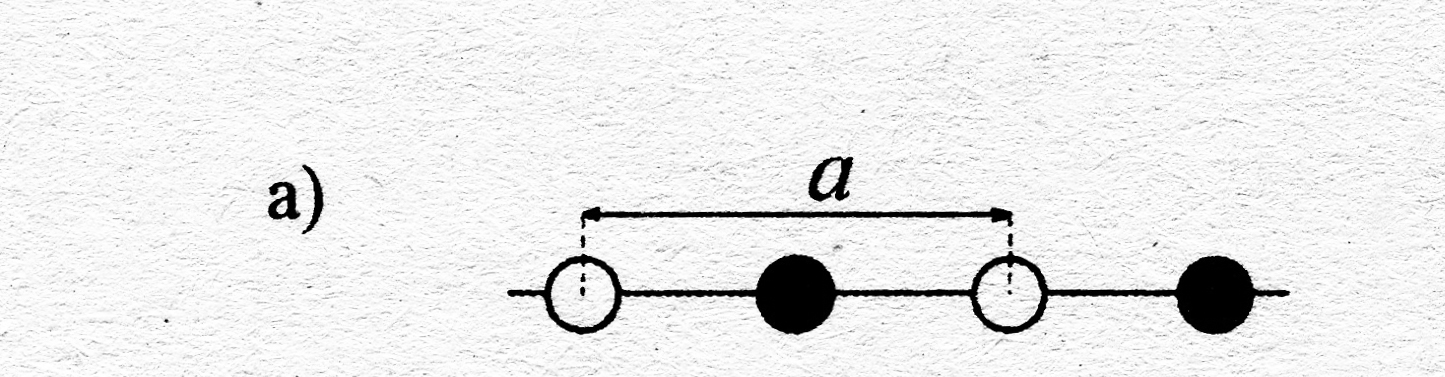
\includegraphics[width=\linewidth]{fig/11a}
	\caption{а) линейная цепочка с базисом из двух различных атомов}
	\label{fig:1.1a}
\end{minipage}
\hfill
\begin{minipage}[h]{0.45\linewidth}
	\centering
	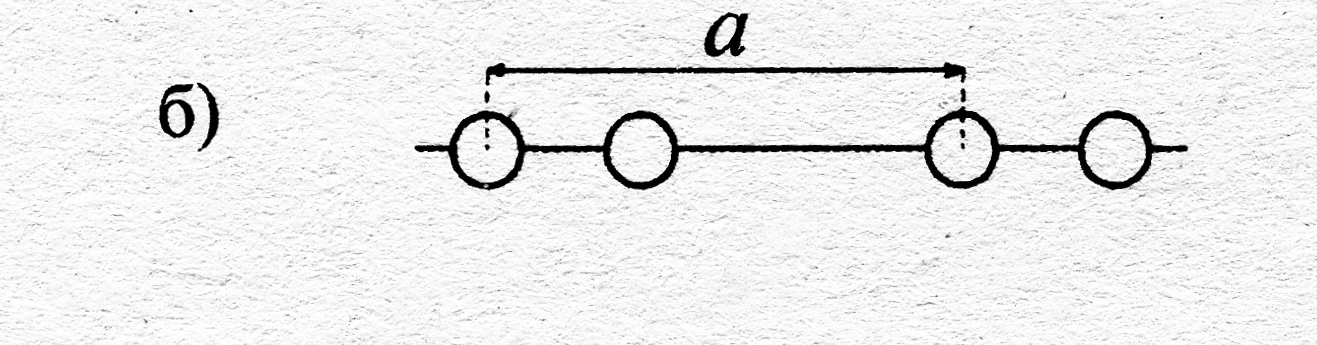
\includegraphics[width=\linewidth]{fig/11b}
	\caption{б) линейная цепочка с базисом из двух одинаковых атомов, при котором возникают оптические колебания}
	\label{fig:1.1b}
\end{minipage}
\vfill
\begin{minipage}[h]{0.45\linewidth}
	\centering
	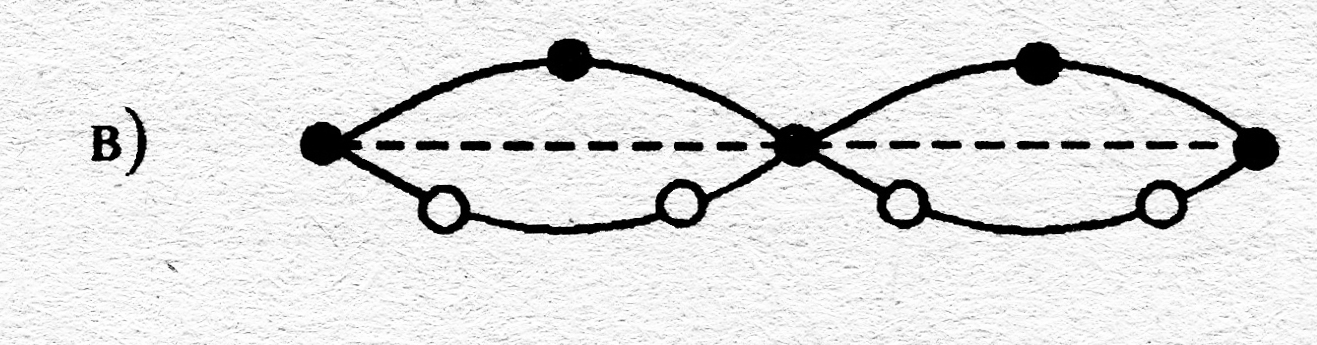
\includegraphics[width=\linewidth]{fig/11c}
	\caption{в) поперечные оптические колебания в линейной цепочке}
	\label{fig:1.1c}
\end{minipage}
\hfill
\begin{minipage}[h]{0.45\linewidth}
	\centering
	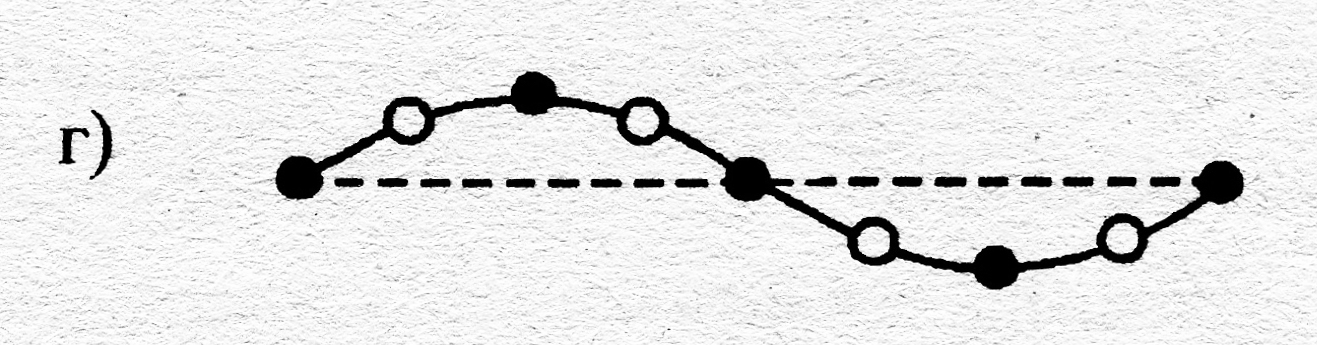
\includegraphics[width=\linewidth]{fig/11d}
	\caption{акустические колебания}
	\label{fig:1.1d}
\end{minipage}
\end{figure}

Колебания более высокой частоты $\omega_1$  принято называть \textit{оптическими}, а 
с $\omega_2$-акустическими. При $q\rightarrow 0$ в оптической ветви колебаний атомы 
решетки смещаются в противоположных направлениях, т.е. колеблются в противофазе, так что
центр тяжести каждой пары, составляющей ячейку, остается неподвижным
(рис. \ref{fig:1.1c}). В акустической же ветви атомы смещаются в одну сторону
(рис. \ref{fig:1.1d}). На рис. \ref{fig:2} изображены соответствующие дисперсионные кривые колебаний.
\begin{figure}[h!]
	\centering
	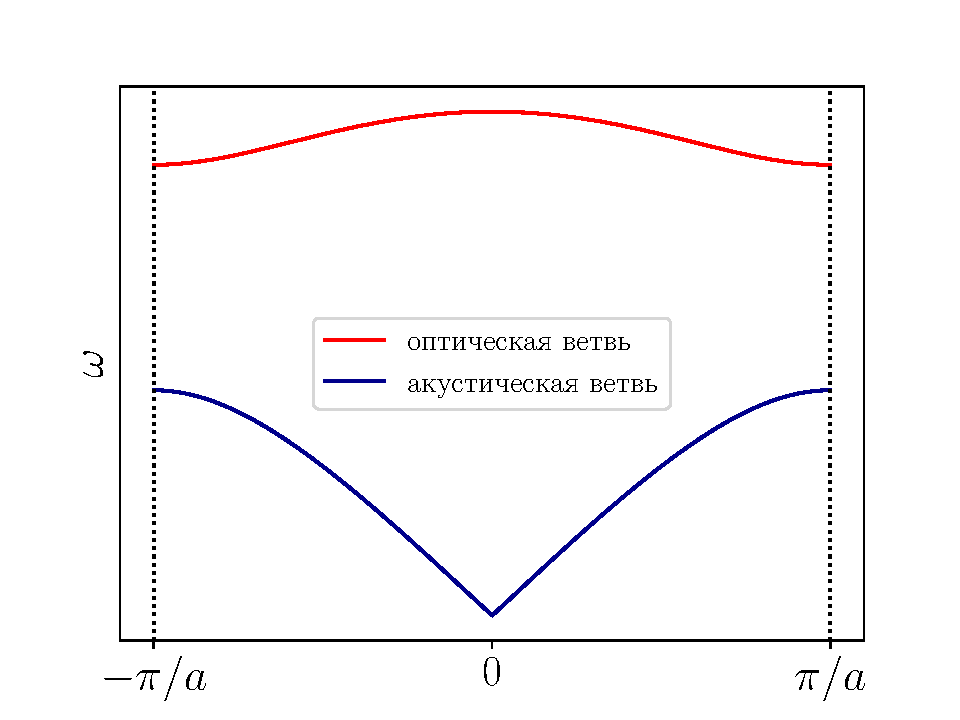
\includegraphics[width=0.5\linewidth]{fig/fig1_2}
	\caption{Дисперсионные кривые тепловых колебаний кристаллической решетки}
	\label{fig:2}
\end{figure}

Заметим, что выводы теории для линейной цепочки с чередующимися атомами разных масс в определенном смысле пригодны и для линейной цепочки с одинаковыми атомами, при условии, что имеются две подрешетки (рис. \ref{fig:1.1b}). В элементарной ячейке цепочки, изображенной на \ref{fig:1.1b} содержатся два атома. Оптические колебания возникают 
в результате колебания в противофазе одной подрешётки  относительно другой. В объёмном кристалле сохраняются основные закономерности, справедливые для одномерной решетки. Поэтому оптические колебания наблюдаются, в частности, в $Si$ и $Ge$, которые сдержат один
сорт атомов, но состоят из двух подрешеток (структура типа алмаза). Однако,
для объемных кристаллов, имеющих в алиментарной ячейке только один атом,
как и для простых (однородных) линейных цепочек, существуют только акустические колебания.

Энергия каждого нормального колебания квантована. Нормальные колебания  можно рассматривать подобно линейным гармоническим осцилляторам с собственной частотой $\omega_{qj}$ и энергией
\begin{equation}
	W_{qj}=\hbar \omega_{qj}\qty(n_{qj}+\frac12),
\end{equation}
где $n_{qj}=0,1,2,\dots$-- главное квантовое число $qj-$го осциллятора, колеблющегося с частотой
$\omega_{qj}$, j - индекс ветви колебаний. 

Полная энергия теплового движения атомов складывается из энергий всех нормальных колебаний
\begin{equation}
	W=\sum_{q,j} W_{qj}=\sum_{q,j} \hbar \omega_{qj} (n_{qj}+\frac12),
\end{equation}
где волновое число $q$ имеет столько разрешенных значений, сколько в кристалле
элементарных ячеек. При описании взаимодействия носителей заряда с тепловыми колебаниями решётки принято говорить о квазичастицах - фононах носителях квантов энергии колебаний решетки. При таком подходе изменение энергии колебаний решётки на один квант рассматривается как появление (или исчезновение) одного фонона с энергией и импульсом $ p = \hbar q$ . Процесс
рассеяния электронов на тепловых колебаниях решетки теперь можно рассматривать как столкновение с фононом. При таком столкновении должны соблюдаться законы сохранения энергии и импульса 
\begin{equation}
	\label{eq:lse}
	\vec k' = \vec k \pm \vec q, ~ W'= W\pm \hbar \omega_{qj},
\end{equation}
где $\vec k$, $\vec q$ - волновые векторы электрона и фонона до столкновения; $\vec k'$ - волновой вектор электрона после столкновения; $W$ и $W'$ - соответственно, энергия электронов до и после столкновения. Процесс, соответствующий в \eqref{eq:lse} знаку плюс, интерпретируется как поглощение, а знаку минус -- испускание электроном фонона.

В некоторых отношениях фононы ведут себя не так, как обычные частицы. Во-первых, среднее число фононов зависит от температуры, а во-вторых, при взаимодействии, например, с электронами или друг с другом фононы возникают и исчезают. Поэтому их называют квазичастицами.

\subsubsection{Дрейф электрона во внешнем электрическом поле}


Рассмотрим движение электрона в реальном полупроводнике во внешнем электрическом поле. Так как в реальной кристаллической структуре присутствуют дефекты частица движется ускоренно лишь на небольшом участке пути, а затем испытывает рассеяние, теряет направленную скорость, псле чего процесс разгона начинается заново. Движение электрона между актами рассеяния по прежнему описывается уравнениями  \eqref{eq:1.4a} и \eqref{eq:1.4b}. Если время свободного пробега электрона (время между двумя процессами рассеяния) мало по сравнению со временем движения электрона от одного края зоны Бриллюэна до другого, то эффективная масса электрона мало меняется во время его свободного пробега. Тогда зависимость проекции мгновенной скорости электрона на ось, направленную против внешнего электрического поля представлена на рис. \ref{fig:3}. Линейный участок на графике соответствует ускорению электрона во внешнем поле, вертикальный -- рассеянию электрона. Благодаря наличию внешнего поля электрон обладает средней скоростью направленного движения вдоль поля, которая называется \textit{дрейфовой скоростью}.

В слабых электрических полях дрейфовая скорость пропорциональна напряженности электрического поля:
\begin{equation}
\label{eq:1.14}
	v=\mu E
\end{equation}

\begin{figure}[h!]
	\centering
	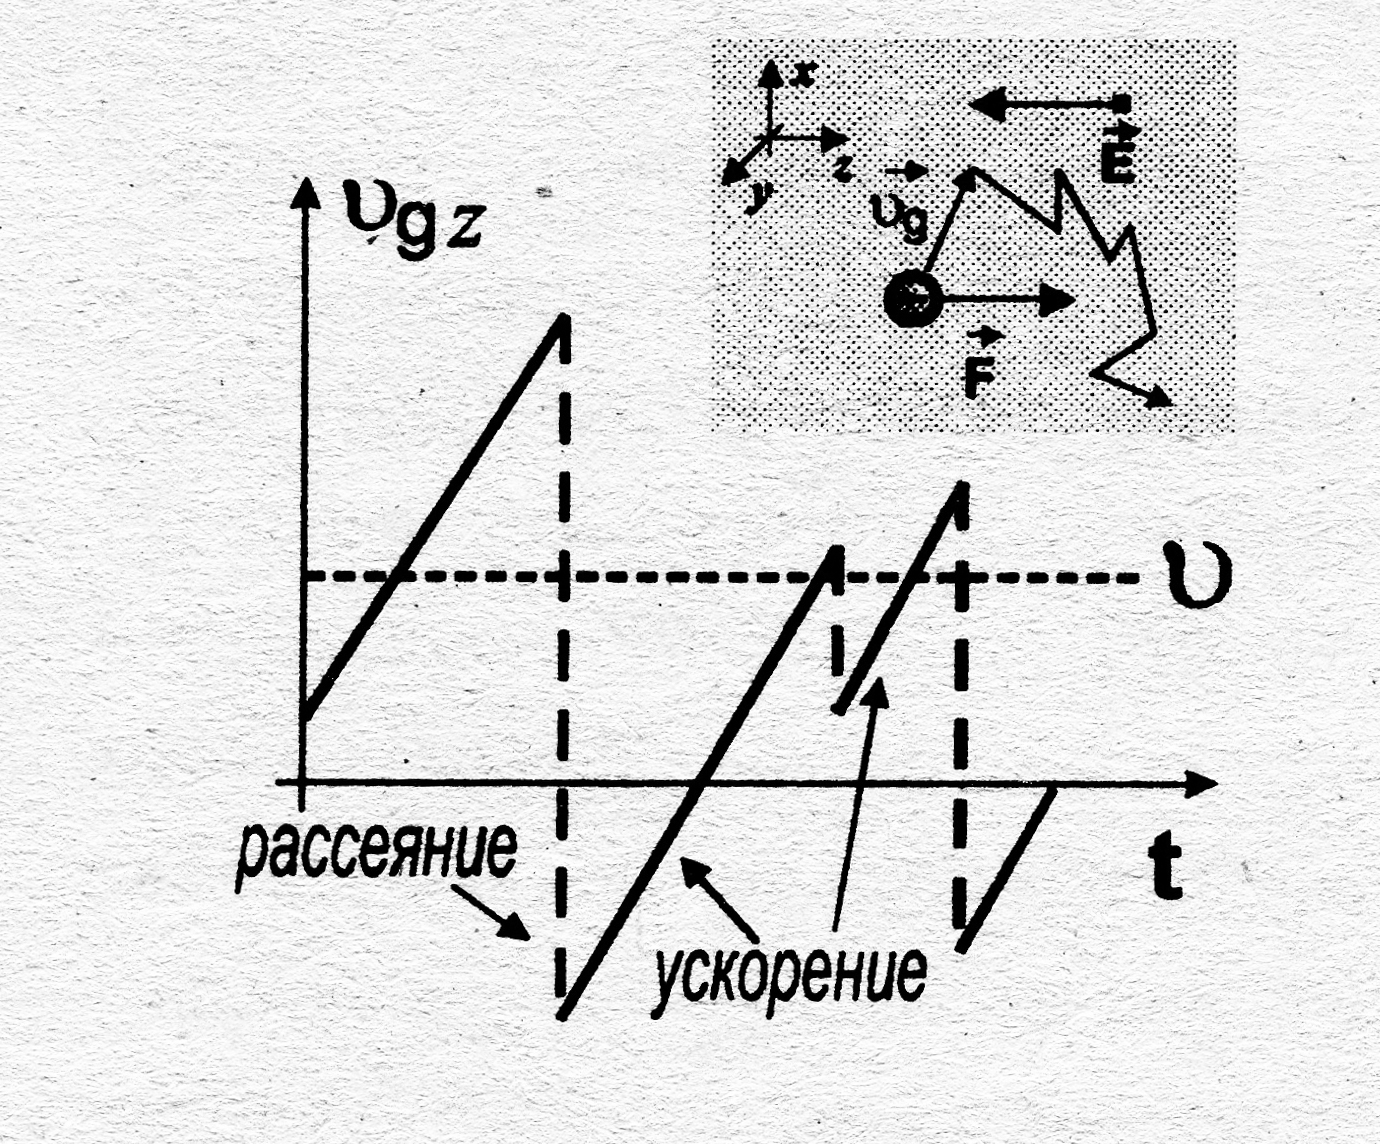
\includegraphics[width=0.5\linewidth]{fig/13}
	\caption{Зависимость проекции мгновенной скорости носителей заряда от времени}
	\label{fig:3}
\end{figure}

Коэффициент пропорциональности между скоростью и полем $\mu$ называется подвижностью носителей заряда . Эта величина численно равна средней скорости
направленного движения частиц в электрическом поле с единичной напряженностью.

Интересно, что при увеличении электрического поля дрейфовая скорость
перестает расти по линейному закону и в больших полях или стремится к установившемуся значению или уменьшается. Типичные зависимости скорости
дрейфа носителей заряда в различных полупроводниках приведены на рис.\ref{fig:4}

\begin{figure}[h!]
	\centering
	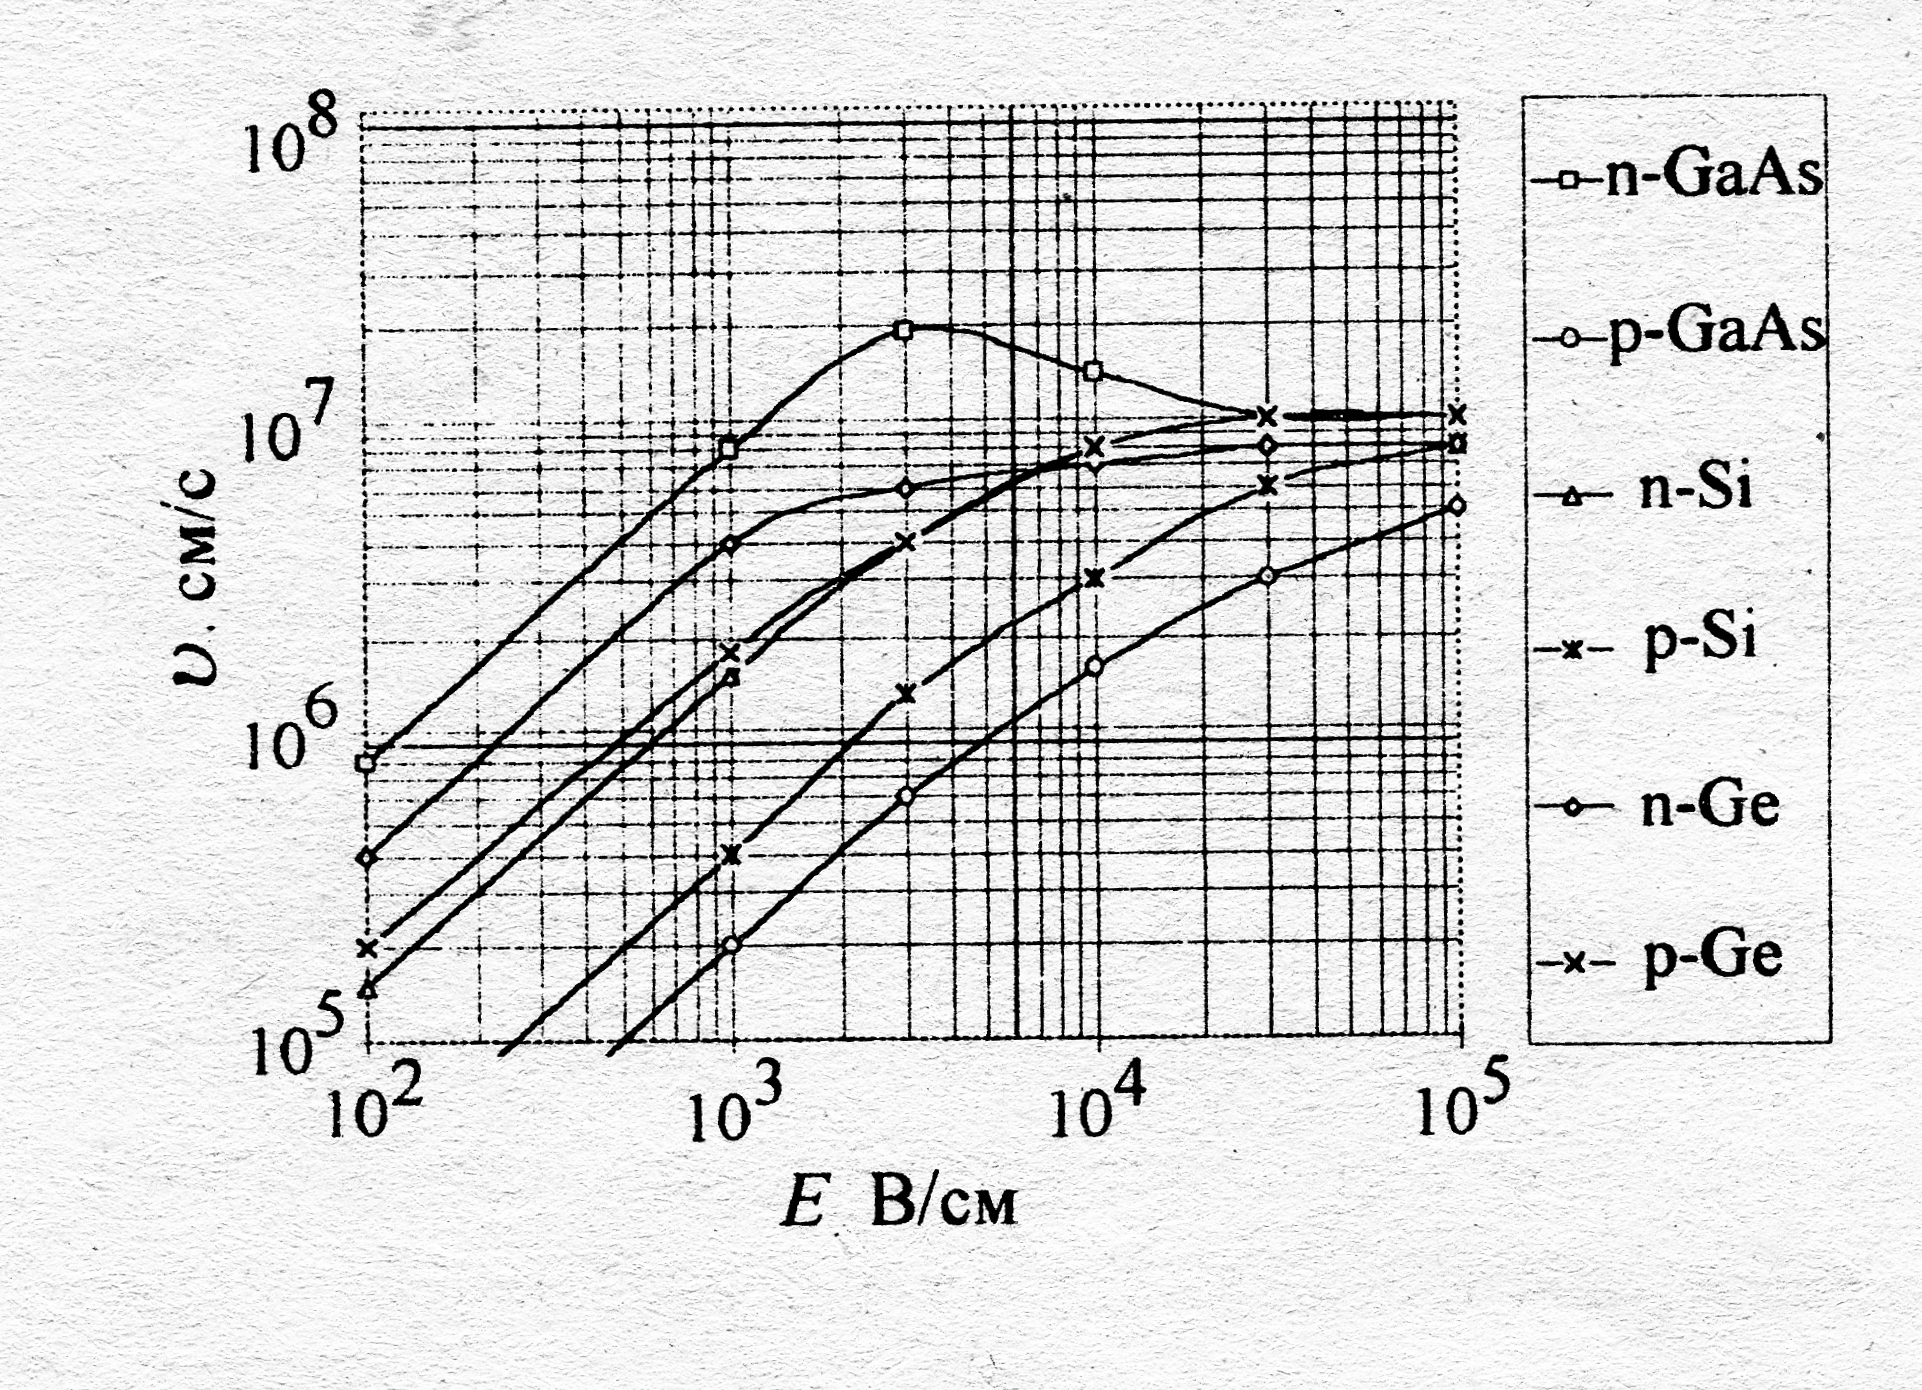
\includegraphics[width=0.5\linewidth]{fig/14}
	\caption{Экспериментальные зависимости дрейфовой скорости носителей зарада от напряженности электрического поля для $Ge$, $Si$, $GaAs$}
	\label{fig:4}
\end{figure}

Характер зависимости $v(E)$ определяется как структурой зоны проводимости полупроводника, так и механизмами рассеяния. В валентных материалах основной причиной ограничения дрейфовой скорости является рассеяние на оптических фононах. В отличие от почти упругого рассеяния на акустических фононах, рассеяние на оптических фононах является резко неупругим, т. е. про­
исходит существенное изменение энергии носителей заряда. Как только энергия
электрона становится выше энергии оптического фонона (см. рис. \ref{fig:2}), резко
возрастает количество актов столкновений, сопровождающихся возбуждением
фонона. Таким образом, электрон активно отдаёт энергию кристаллической
решетке, что препятствует дальнейшему росту скорости его направленного движения. В режиме насыщения скорости вся энергия, набираемая электроном в электрическом поле за время свободного пробега, отдаётся им в кристаллическую решётку посредством возбуждения фононов.

В полупроводниковых соединениях ($GaAs$, $InP$ и др.) на зависимость сред­ней скорости электронов от напряженности электрического поля существенно влияет переход электронов из $\Gamma$-долины с низкой эффективной массой носителей
заряда в верхние $L$ и $X$ долины со значительно большей массой и меньшей подвижностью (средней дрейфовой скоростью) электронов \cite{lit4}-\cite{lit5}. Как правило, такой
процесс происходит при столкновении с оптическим фононом. После столкновения направленная скорость электрона в среднем теряется. В результате этих
процессов на зависимости средней скорости электронов от напряженности электрического поля появляется экстремум, а количество электронов, находящихся в
верхних долинах, (заселенность долин) растет с увеличением напряженности по­
ля.

\subsubsection{Движение носителей зарядка в плавно изменяющихся во времени или в пространстве электрических полях}


Наиболее общей системой уравнений, описывающей перемещение во
внешнем электрическом поле ансамбля электрически заряженных частиц в случае, когда электрические поля медленно меняются во времени\footnote{по сравнению со временем релаксации энергии электронов $\tau_W$} или в пространстве\footnote{по сравнению с длиной релаксации энергии электронов $l_W=\tau_W\cdot v_T$, где $v_T$-- тепловая скорость электрона при температуре T}, является система уравнений, включающая в себя

\begin{itemize}
	\item \textbf{уравнение Пуассона} (полученное из предположения о малости скорости дрейфа носителей заряда в полупроводниковом материале по сравнению со скоростью света, когда справедливо выражение $\vec E=-\nabla \varphi $)
\begin{equation}
	\label{eq:1.15}
	\Delta \varphi =- \frac{1}{\epsilon \epsilon_0} \rho(x,y,z),
\end{equation}
 где $\vec E$ - напряженность электрического поля, $\varphi$- потенциал, $\epsilon$-диэлектрическая проницаемость материала, $\rho(x,y,z)$- объемная плотность зарядка (включает в себя подвижные заряды электронов и дырок, а также неподвижные заряженные структурные дефекты полупроводника, в том числе, ионизированные примеси);

 	\item \textbf{выражения для плотности электронного и дырочного токов}

 	\begin{gather}
 		\vec j_n = -en \vec v_n + e\cdot \nabla(D_n n) \\ 
 		\label{eq:1.16a}
 		\vec j_p = ep \vec v_p - e\cdot \nabla(D_p p), \\
 		\label{eq:1.16b}
 	\end{gather}
 	n,p - концентрации, а $\vec v_n$ $\vec v_p$ - дрейфовые скорости электронов и дырок, соответственно; $e$- абсолютная величина заряда электрона; $D_n$, $D_p$- коэффициенты диффузии носителей заряда; каждое из выражений \eqref{eq:1.16b} и \eqref{eq:1.16a} для плотности тока содержит \textit{дрейфовую} (которая определяется движением носителей в электрическом поле) и \textit{диффузионную} (которая возникает из-за теплового движения подвижных зарядов) составляющие.

 	\item \textbf{уравнения непрерывности для электронов и дырок}, которые в отсутствие генерации и рекомбинации частиц записываются в виде
 	\begin{equation}
 		\label{eq:1.17}
 		\pdv{n}{t}=\frac{1}{e}\div{\vec j_n}, ~ \pdv{p}{t}=-\frac{1}{e}\div{\vec j_p}
 	\end{equation}

\end{itemize}
 	Система уравнений \eqref{eq:1.15}-\eqref{eq:1.17} дополняется \textit{соотношением Эйнштейна}, описывающим связь между подвижность и коэффициентом диффузии
 	\begin{equation}
 		D=\frac{kT}{e}\mu
 	\end{equation}
 	и выражением для дрейфовой скорости носителей зарядка как функции электрического поля
 	\begin{equation}
 		v_n=v_n(E) \text{ и } v_p=v_p(E)
 	\end{equation}
 	Тогда выражение для полной плотности тока в полупроводнике записывается в виде
 	\begin{equation}
 		\vec j = \vec j_n +\vec j_p +\pdv{E}{t},
 	\end{equation}
 	где третье слагаемое описывает ток смещения.


 	\subsubsection{Движение носителей заряда в резко изменяющихся во времени или пространстве электрических полях}


Для описания движения носителей заряда в полупроводниковых структурах при резко изменяющихся полях используется система уравнений, которая,
помимо уравнений \eqref{eq:1.15} - \eqref{eq:1.17} включает в себя уравнение баланса импульса
\eqref{eq:1.23}, уравнение баланса энергии \eqref{eq:1.24} и выражение для плотности потока
энергии \eqref{eq:1.26}. В случае транспорта электронов полная система уравнений имеет
следующий вид:
\begin{gather}
	\label{eq:1.21}
	\Delta  \varphi = -\frac{e}{\epsilon \epsilon_0} \qty(N_d-n)  \\
	\label{eq:1.22}
	\pdv{n}{t}=\frac{1}{e} \div{\vec j_n}\\
	\label{eq:1.23}
	\dv{ \qty (m^*\vec v) }{t}= -e\vec E - \frac{m^*}{\tau_p} \vec v \\
	\label{eq:1.24}
	\pdv{(Wn)}{t}=\div{\vec j_W}+ \qty(\vec j_n, \vec E)-\frac{n\qty(W-W_0)}{\tau_W} \\
	\label{eq:1.25}
	\vec j_n = - en\vec v + e\cdot \grad{(D_n n)} \\
	\label{eq:1.26}
	\vec j_W= -nW \vec v +\grad{(D_n n W)} \\ 
	\label{eq:1.27}
	\vec j = \vec j_n + \pdv{\vec E}{t} \\
	\label{eq:1.28} 
	\vec{E}=-\grad{\varphi}
\end{gather}
Здесь $N_d$ - концентрация доноров; 
$m^*$- эффективная масса электронов;
$\vec j_W$- плотность потока энергии электронов;
$\tau_p, \tau_W$- \textit{времена релаксации} импульса и энергии носителей;
$W_0=\frac32 kT$- средняя тепловая энергия электронов.

Уравнения баланса \eqref{eq:1.26} и \eqref{eq:1.24} выражают, по сути, законы сохранения
импульса и энергии частиц. Импульс направленного движения электронов может
увеличиваться за счет разгона в электрическом поле (первое слагаемое в правой
части \eqref{eq:1.23} и уменьшаться из-за рассеяния носителей на дефектах структуры
(второе слагаемое). Энергия носителей в некотором замкнутом объеме, помимо
тех же причин, может изменяться за счет втекания или вытекания горячих (т е.,
высокоэнергетических) или холодных носителей, что отражает первое слагаемое
в правой части \eqref{eq:1.24}.
В стационарном состоянии $\dv{(m^*v)}{t}=0, ~ \pdv{W}{t}=0$ уравнения \eqref{eq:1.23} и
\eqref{eq:1.24} принимают следующий вид:
\begin{gather}
	\label{eq:1.29}
	\tau_p=\frac{m^*v_s}{eE} \\
\label{eq:1.30}
	\tau_W=\frac{W_s-W_0}{eEv_s},
\end{gather}

где индекс <<s>> означает стационарное значение. Выражения \eqref{eq:1.29}, \eqref{eq:1.30}
связывают времена релаксации со стационарными значениями скорости и энергии.
Время релаксации по импульсу, как правило, много меньше времени релаксации
по энергии, т.к. упругие столкновения не изменяют энергию, но могут существенно изменить импульс частицы. На рис. \ref{fig:5} приведены графики зависимости
времени релаксации энергии и импульса в кристаллах $Si$ и $GaAs$ от величины
средней энергии носителей заряда.
\begin{figure}[h!]
	\centering
	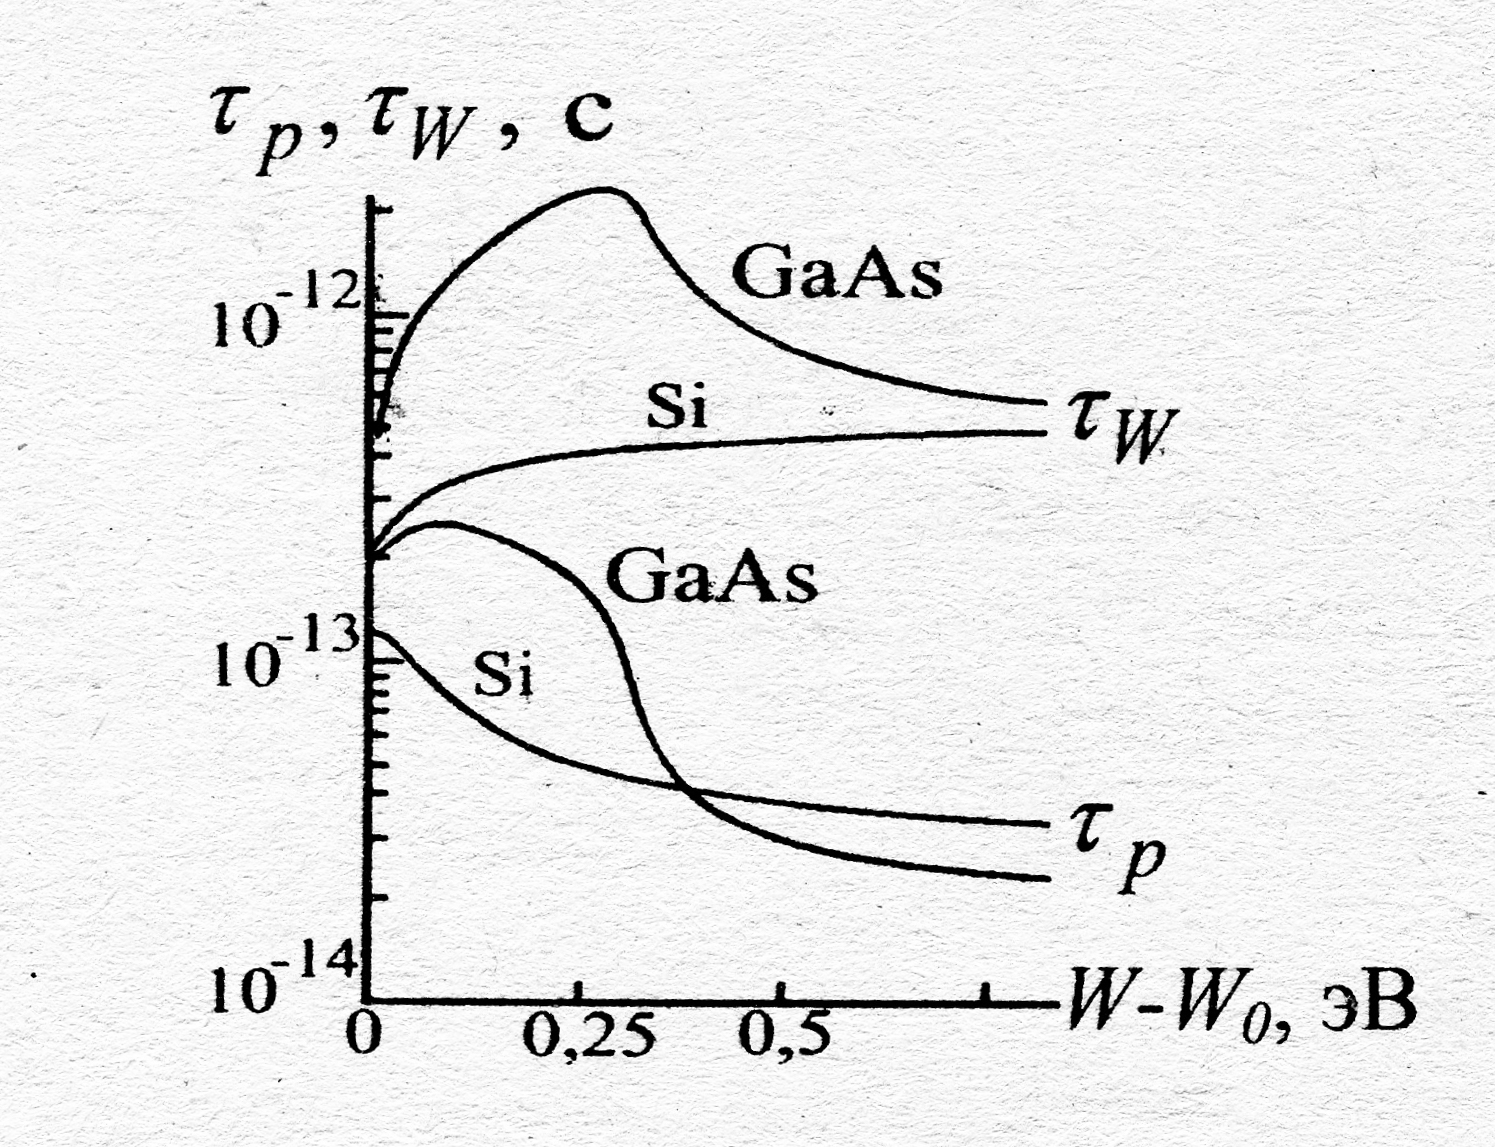
\includegraphics[width=0.7\linewidth]{fig/15}
	\caption{Зависимость времени релаксации энергии и импульса от разницы между средней 
	($W$) и тепловой энергией ($W_0$) электронов в кристаллах $Si$ и $GaAs$}
	\label{fig:5}
\end{figure}
Из \eqref{eq:1.14} и \eqref{eq:1.29} следует, что 
\begin{equation}
\label{eq:1.31}
	\mu =\frac{e \tau_p}{m^*}
\end{equation}
Даже в случае полупроводников с высокой подвижностью носителей заряда,
максимальная стационарная дрейфовая скорость частиц не превышает I-
$3\cdot 10^7\frac{\text{см}}{\text{с}}$, что, казалось бы, накладывает принципиальное ограничение на быстродействие твердотельных приборов. Однако в динамическом режиме и в коротких образцах можно получить дальнейшее увеличение дрейфовой скорости электронов. Суть этого явления состоит в следующем. Когда носители попадают в
область резкого скачка поля, скорость направленного движения начинает быстро
расти у всех частиц одновременно. Поэтому средняя скорость носителей заряда в
течение короткого периода времени может быть существенно выше ее стационарного значения (\textit{эффект всплеска скорости во времени}). Затем столкновения электронов с дефектами структуры приводят к сбросу средней скорости частиц и через некоторое время (порядка нескольких времен релаксации импульса) устанавливается стационарное значение средней по ансамблю скорости носителей для данного значения поля. Таким образом, если не <<дожидаться>>
установления стационарной скорости, а использовать нестационарное значительное увеличение дрейфовой скорости частиц на временах $\sim \tau_p$, то можно получить значительное увеличение дрейфовой скорости частиц, что существенно сказывается на параметрах полупроводниковых приборов. На рис. \ref{fig:6} приведены расчетные зависимости $v(t)$ для 
$GaInAs$\footnote{$GaInAs$ -- тройное полупроводниковое соединение, отличающиеся от $GaAs$ тем, что часть атомов галлия замещена индием}, $InP$  и $GaAs$.
\begin{figure}[h!]
	\centering
	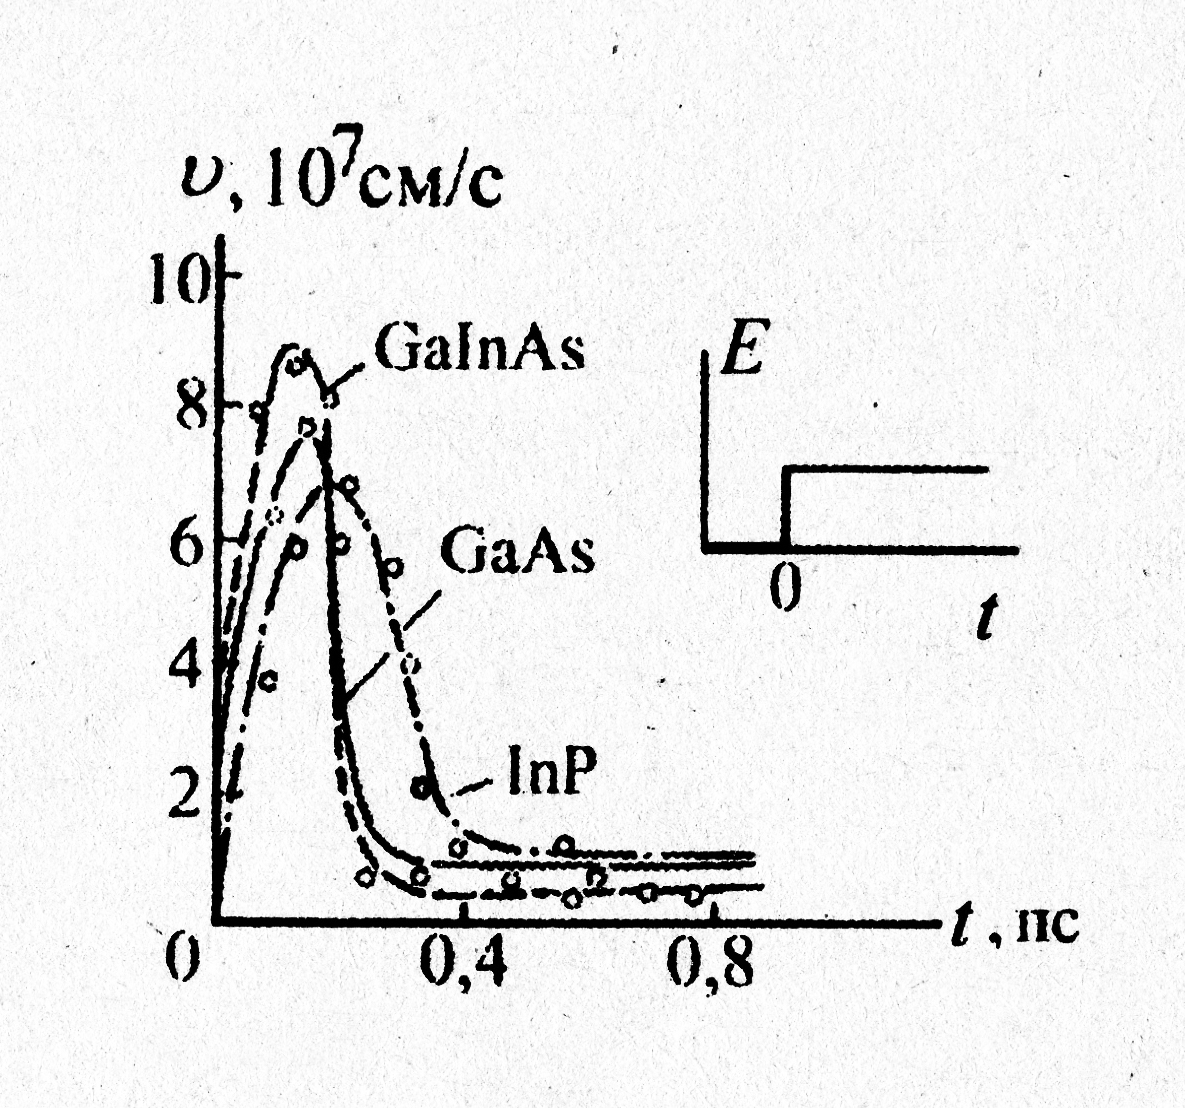
\includegraphics[width=0.7\linewidth]{fig/16}
	\caption{Изменение дрейфовой скорости электронов во времени после мгновенного включения электрического поля $E=40$ кВ/см. Кривые и точки соответствуют различным методам счета \cite{lit6}}
	\label{fig:6}
\end{figure}

Характерные размеры активной области современных диодов и транзисторов имеют значения порядка 10-100 нм. В таких условиях длина прибора может стать сравнимой со средней длиной свободного пробега носителей в полупроводнике, а время пролета может оказаться примерно равным или меньше среднего времени релаксации энергии и импульса носителей заряда. В таких условиях равновесное распределение носителей не успевает установиться, и средняя дрейфовая скорость электронов во всей активной области прибора может существенно превосходить значения насыщенной скорости в длинных образцах. Это увеличение скорости за счет нестационарных эффектов получило название \textit{эффект всплеска скорости в пространстве}. На рис. \ref{fig:7} приведены рассчитанные максимальные значения дрейфовой скорости для коротких образцов $GaAs$. Как видим, даже у образцов 300-500 нм величина скорости остается много больше максимального стационарного значения $v_s \approx 3\cdot 10^7$ см/с.
\begin{figure}[h!]
	\centering
	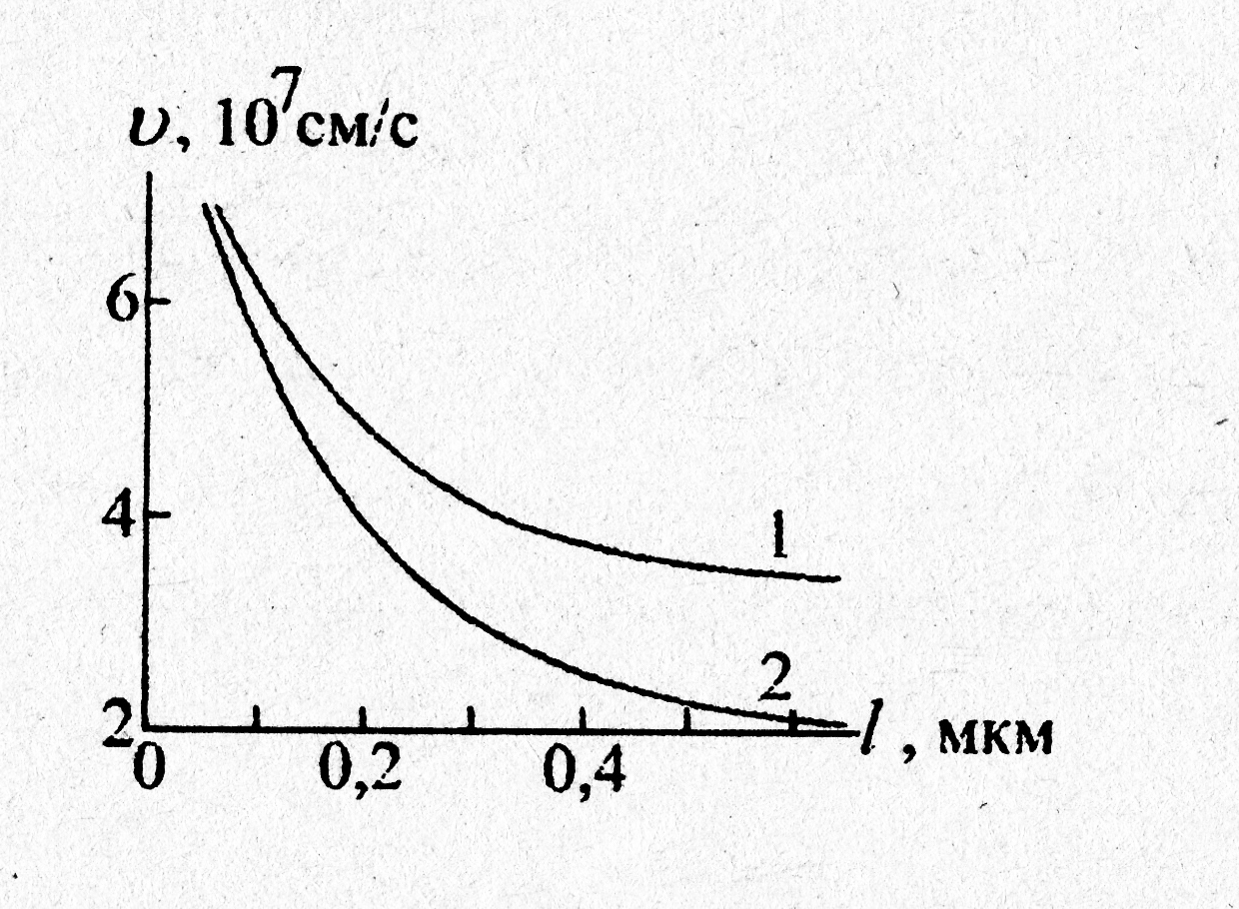
\includegraphics[width=0.7\linewidth]{fig/17}
	\caption{Зависимости максимального значения средней дрейфовой скорости в образцах с различной длиной l, рассчитанные для $GaAs$ при двух значениях концентрации примеси: 1- $N_d=0$; 2 - $N_d=3\cdot 10^{17} \text{см}^{-3}$. $T=293 K$}
	\label{fig:7}
\end{figure}

В многодолинных полупроводниках, как и в стационарном случае, на динамику дрейфовой скорости на коротких отрезках времени существенно влияет междолинного переброса. Если в многодолинных материалах эффект всплеска скорости обычно сопровождается переходом в верхние долины, то в полупроводниках типа $Si$ и $Ge$ всплеск скорости не так явно выражен, но тем не менее, увеличение скорости может составлять 1.5-3 раза.

\subsection{Элементарная теория эффекта Холла}
Анализ транспорта носителей в полупроводниковых структурах, представленный в предыдущем разделе, требует знания концентрации носителей заряда и их подвижности в материале. Эти характеристики являются важными физическими величинами, определяющими многие свойства полупроводников, например, электропроводность, теплопроводность, термо-ЭДС и др.

Концентрацию и подвижность в отдельности можно определить, зная соотношение между ними. В данной работе это соотношение устанавливается экспериментально при помощи эффекта Холла.

Эффект Холла представляет собой поперечный гальваномагнитный эффект, суть которого заключается в следующем: если поместить полупроводниковую пластину во внешнее магнитное поле $\vec B$ (рис. \ref{fig:8}) и пропустить вдоль нее ток, то вследствие смещения движущихся зарядов к одной из граней пластины возникает поперечная разность потенциалов, называемая \textit{ЭДС Холла}. При этом (см. рис. \ref{fig:8}.б, \ref{fig:8}.в), носители различных знаков смещаются к одной и той же боковой грани полупроводника, поэтому с изменением типа электропроводности меняется и знак ЭДС.

С помощью эффекта Холла можно экспериментально определить тип носителей, концентрацию и подвижность в данном полупроводниковом образце. Другим важным практическим приложением этого эффекта являются измерения силы тока и мощности в цепях постоянного и переменного тока  (вплоть до очень высоких частот), напряженности постоянных и переменных магнитных полей, преобразование сигналов, анализ спектров и т.д.

\begin{figure}[h!]
	\centering
	\includegraphics[width=\linewidth]{example-image-a}
	\caption{Возникновение ЭДС Холла: схема эксперимента (а); смещение носителей заряда в дырочном (б) и электронном (в) полупроводниках, соответственно}
	\label{fig:8}
\end{figure}

Разберем эффект Холла более подробно. На рис. \ref{fig:8}.а показан полупроводник, две плоскости которого подключены через омические (т.е. невыпрямляющие) контакты к внешней батарее. Обозначим $\vec j$ плотность тока в направлении Ox. Магнитное поле $\vec B$ приложено в направлении Oy. Рассмотрим электрон, двигающийся в отрицательном направлении оси Ox со средней скоростью $\vec V$. На движущийся в магнитном поле электрон действует магнитная составляющая силы Лоренца:
$$\vec F = -e [\vec v, \vec B].$$
В результате действия этой силы траектория электрона будет искривляться  в направлении оси z, и, поскольку в этом направлении ток протекать не может, электроны будут накапливаться на боковой поверхности ($z=\pm a$, см. рис. \ref{fig:8}) до тех пор, пока не установится электрическое поле $\vec E_H$, достаточное для создания силы. равной магнитной составляющей силы Лоренца, но направленной противоположно. Приравнивая эти силы, получим: 
\begin{equation}
\label{eq:2.1}
	\vec E_H=[\vec v, \vec B]
\end{equation}

Воспользуемся законом Ома в дифференциальной форме:
\begin{equation}
\label{eq:2.2}
	\vec j = \sigma \vec E,
\end{equation}
где $\sigma = e \cdot n \cdot \mu_n$ - удельная проводимость образца, $\mu_n = \frac{v}{E}$ - подвижность носителей. Соотношение \eqref{eq:2.2} перепишем в следующем виде:
\begin{equation}
\label{eq:2.3}
	\vec j = e \cdot n \cdot \mu_n \cdot \vec E = -e \cdot n \cdot \vec v
\end{equation}

Исключая $v$ из соотношения \eqref{eq:2.1}, получим:
\begin{equation}
\label{eq:2.4}
	\vec E_H = -\frac{1}{en} [\vec j, \vec B]=R[\vec j, \vec B]
\end{equation}

Учитывая, что полный ток через образец $I=jab$, а поперечная ЭДС $U_H=E_Ha$, получим соотношение, связывающее ЭДС Холла с величиной электрического тока:
\begin{equation}
\label{eq:2.5}
	U_H=R \cdot \frac{I\cdot B}{b}
\end{equation}

Величина R называется \textit{постоянной Холла} и определяется как

\begin{equation}
\label{eq:2.6}
	R=-\frac{1}{e\cdot n}
\end{equation}

Поперечную ЭДС $U_H$, ток I, напряженность магнитного поля B (для немагнитных образцов) и толщину b полупроводникового образца можно измерить. Это позволяет найти численное значение постоянной Холла.

В действительности, произведенный элементарный вывод коэффициента Холла \eqref{eq:2.6} неточен: в нем не учтена разница между мгновенной скоростью электронов, входящей в выражение магнитной составляющей силы Лоренца, и дрейфовой скоростью, которую электрон приобретает под действием электрического поля. Кроме того, не учитывается распределение электронов по скоростям и механизмы рассеяния носителей. Формула \eqref{eq:2.6} оказывается справедливой только для металлов и вырожденных полупроводников (вырожденным называется полупроводник с очень высокой, порядка $10^{19}$ атом/$\text{см}^3$, концентрацией примеси). Более строгий анализ дает для невырожденных полупроводников значение R, которое отличается от выражения \eqref{eq:2.6} множителем А. Если учитывать рассеяние носителей только на кристаллической решетке (взаимодействие с фононами), то $A=\frac{3\pi}{8}$. В общем виде постоянная Холла может быть записана как:
\begin{gather}
	R=-\frac{A}{n\cdot e} \text{(для полупроводника n-типа)} \notag \\
	R=\frac{A}{p\cdot e} \text{(для полупроводника p-типа)}
\label{eq:2.7}
\end{gather}
где множитель А может принимать значения от 1 до 1.7. Знак минус в формуле \eqref{eq:2.7} демонстрирует, что ЭДС Холла для электронного полупроводника имеет полярность, противоположную полярности для дырочного полупроводника.

Знание электропроводности и постоянной Холла позволяет найти как концентрацию носителей, так и их подвижность.

Обозначим через холловский угол $\theta_H$ малый угол, который образует с осью х вектор напряженности суммарного электрического поля (см. рис. \ref{fig:8}):
\begin{equation}
\label{eq:2.8}
	\theta_H \cong \tg{\theta_H}=\frac{E_H}{E}
\end{equation}

Из \ref{eq:2.8} с учетом \ref{eq:2.2} и \ref{eq:2.4} получим:
\begin{equation}
\label{eq:2.9}
	\theta_H = \mu_{nH} \cdot B
\end{equation}
где $\theta_H$-холловский угол в проводнике n-типа, а $\mu_{nH}$ - так называемая \textit{холловская подвижность} электронов (индекс H указывает на метод определения подвижности). Численное значение холловской подвижности может расходиться с величиной подвижности, определенной другими методами (например, прямым способом, основанным на измерении времени распространения носителей тока по полупроводнику на определенное расстояние с известным ускоряющим полем). Последняя называется дрейфовой подвижностью. Дрейфовую подвижность можно определить из выражения \ref{eq:2.4}, если, используя выражение \ref{eq:2.7}, преобразовать его к виду:
\begin{equation}
\label{eq:2.10}
	\vec E_H = -\frac{A}{en}\cdot[\vec j, \vec B]=-A\cdot \mu_{nd} \cdot [\vec E,\vec B],
\end{equation}
где индекс d при $\mu_{nd}$ указывает, что это дрейфовая подвижность электронов.

Из выражений \eqref{eq:2.8}-\eqref{eq:2.10} следует, что для электронов $\mu_{nH}=A\cdot \mu_{nd}$, а для дырок $\mu_{pH}=A\cdot \mu_{pd}$. Используя выражения \eqref{eq:2.2} и \eqref{eq:2.7}, получим:
\begin{equation}
\label{eq:2.11}
	\mu_{(n,p)H}=R\cdot \sigma.
\end{equation}

Приведенные выше выражения относились к полупроводникам, у которых концентрация неосновных носителей пренебрежимо мала по сравнению с концентрацией основных (униполярная проводимость). Расчет постоянной Холла для материала со смешанной проводимостью приводит к формуле:
\begin{equation}
\label{eq:2.12}
	R= \frac{A}{e}\cdot \frac{n\mu^2_{nd}-p\mu^2_{pd}}{(n\mu_{nd}+p\mu_{pd})^2}.
\end{equation}
для собственного полупроводника $(n=p=n_i)$ получим:
\begin{equation}
\label{eq:2.12}
	R= \frac{A}{e}\cdot \frac{\mu^2_{nd}-\mu^2_{pd}}{\mu_{nd}+\mu_{pd})}\cdot \frac{1}{n_i}.
\end{equation}

У собственных полупроводников R обычно отрицательна, т.к. подвижность электронов чаще всего больше подвижности дырок. На рис. \ref{fig:9} показаны зависимости подвижности электронов и дырок от концентрации примесей в наиболее распространенных полупроводниках.

\begin{figure}[h!]
	\centering
	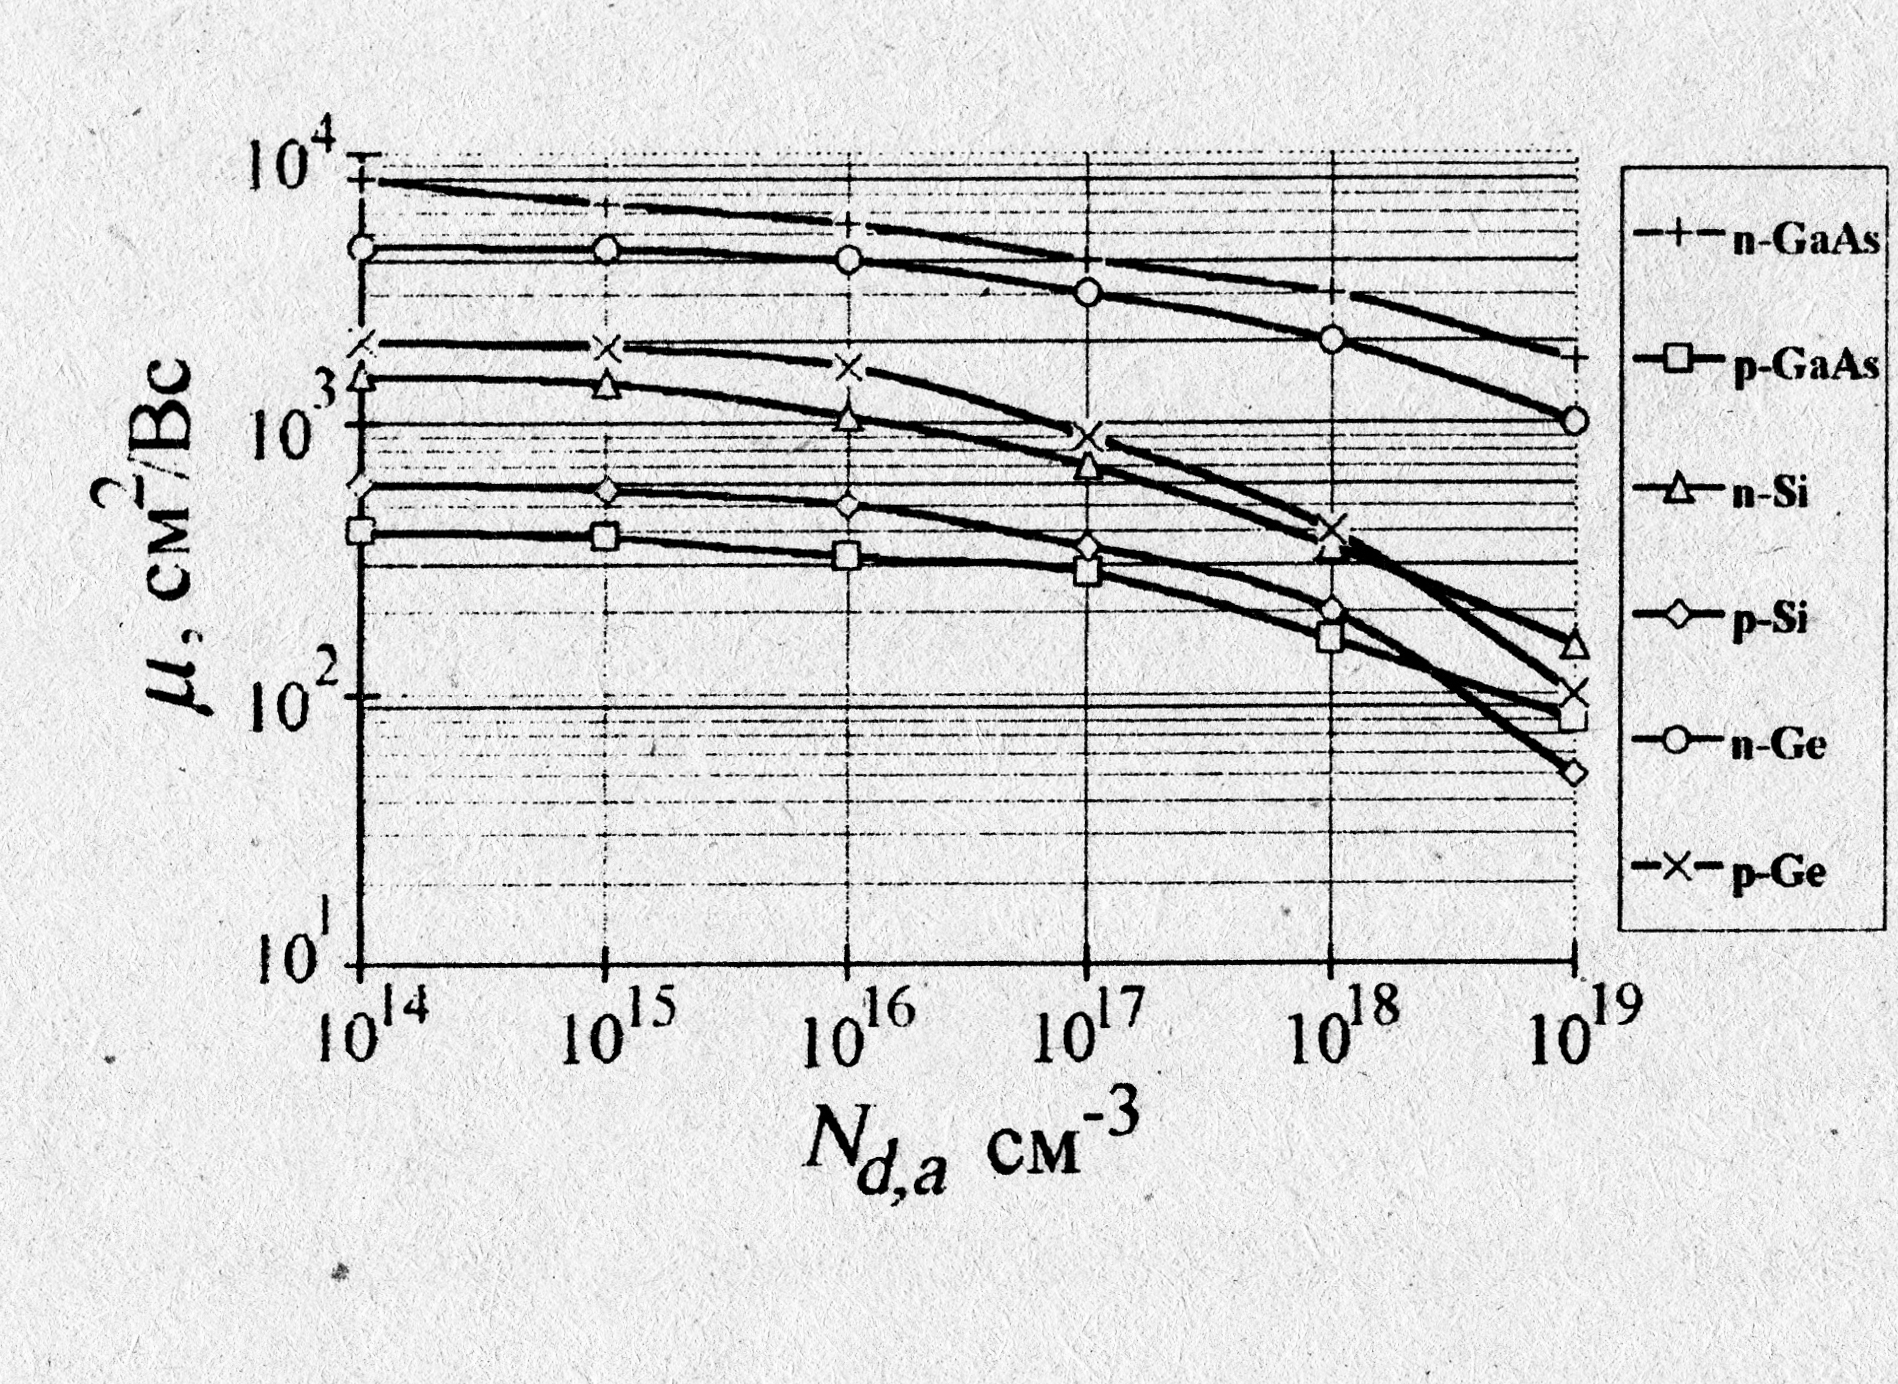
\includegraphics[width=0.7\linewidth]{fig/22}
	\caption{Зависимость дрейфовой подвижности электронов и дырок в $Si$ и $Ge$ и холловской подвижности в $GaAs$ от концентрации атомов легирующей примеси (T=300 K)}
	\label{fig:9}
\end{figure}

% 
% \subsection{Измерительная установка и методика измерений}

% В данной работе измерение постоянной Холла производится на переменном токе (см. блок-схему на рис.\ref{fig:10}). Этот метод дает возможность предельно упростить схему, т.к. использование переменного тока позволяет применять в качестве индикаторов ЭДС Холла широко распространенные измерительные приборы (ламповые вольтметры, осциллографы и др., имеющие достаточно большое входное сопротивление) вместо обычно используемых схем компенсации. Кроме того, при работе на переменном токе легко устраняется паразитная разность потенциалов, которая возникает между холловскими контактами вследствие их несимметричного расположения.

% Схема работает следующим образом: переменное напряжение подается со звукового генератора I через трансформатор Тр, регулировочный потенциометр $R1$, который выведен на переднюю панель установки (на лабораторной установке - ручка "ток образца") и миллиамперметр II подается на образец. Величина тока через образец устанавливается потенциометром $R1$. На одной из боковых поверхностей образца вместо одного холловского контакта установлены два (4,5), потенциал одного из которых заведомо выше, а другого заведомо ниже потенциала 3, расположенного на противоположной поверхности. Потенциометр $R3$ легко позволяет найти точку с потенциалом, равным потенциалу контакта 3, т.е. произвести балансировку холловских контактов. Для этого оправку с образцом устанавливают на опорную площадку вне магнитного поля и, установив ток через образец в пределах 5-6 мА, вращением ручки потенциометра $R3$ (он расположен на оправке) добиваются минимального отклонения луча осциллографа, подключенного вертикальным усилителем к выходному разъему IV установки (усилитель при этом выводится на предельное усиление). После проведения балансировки по осциллографу производится ее проверка на милливольтметре. Балансировка считается удовлетворительной, если сигнал на милливольтметре не превышает 0.5 мВ. 
% \begin{figure}[h!]
% 	\centering
% 	\includegraphics[width=\linewidth]{example-image-a}
% 	\caption{Блок-схема измерительной установки}
% 	\label{fig:10}
% \end{figure}

% После этой проверки оправка с образцом переносится в зазор с магнитным полем и фиксируется на нижнем полюсном наконечнике. При этом надо избегать резких ударов и толчков, т.к. можно сбить балансировку. Выходной разъем V установки служит в качестве источника сигнала, имеющего ту же фазу, что и напряжение на контакте 2 относительно контакта 1. Это опорное напряжение необходимо при определении типа носителей в данном образце. Для определения типа носителей сигнал с выхода IV подается на вертикальный усилитель, а с выхода V - на горизонтальный (при этом ручка осциллографа <<диапазон частот>> должна находится в положении <<выкл.>>). Установив ток через образец 5-7 мА, а усилители осциллографа в режим усиления, наиболее удобный для наблюдения, легко определить разность фаз между контактами 2 и 3 относительно <<земли>>, по которой, зная направление магнитного поля, можно установить тип носителей. Величина магнитного поля может меняться путем изменения расстояния между полюсными наконечниками. 
\section{Практическая часть}
%Внимание!
%Большинство расчетов в данной лабе выполнены pythontex'ом, потому если копируете куски кода, то будьте внимательны к инородному синтаксису :) 
\subsection{Измерение вольт-амперной характеристики образца и его паразитного напряжения}
На рис. \ref{fig:5.2} изображена ВАХ образца. Из графика, зная закон Ома, не трудно установить значение сопротивления $R= \py{round(resistance,2)} \text { Ом}$. 
Зная размеры образца: 
\begin{itemize}
	\item длина $l=\py{l}$ м,
	\item ширина $d=\py{d}$ м,
	\item толщина $b=\py{b} $ м,
\end{itemize}
можем найти его удельное сопротивление $\rho$

\begin{equation}
	\rho = \frexp{rho} ~ \text{Ом}\cdot\text{м},
\end{equation}
а значит и обратную ей величину $\sigma$-- удельную проводимость
\begin{equation}
	\sigma=\frac{1}{\rho}=\frexp{sigma} ~ \frac{1}{\text{Ом}\cdot\text{м}}
\end{equation}

\begin{figure}[h!]
\begin{minipage}[h]{0.49\linewidth}
	\centering
	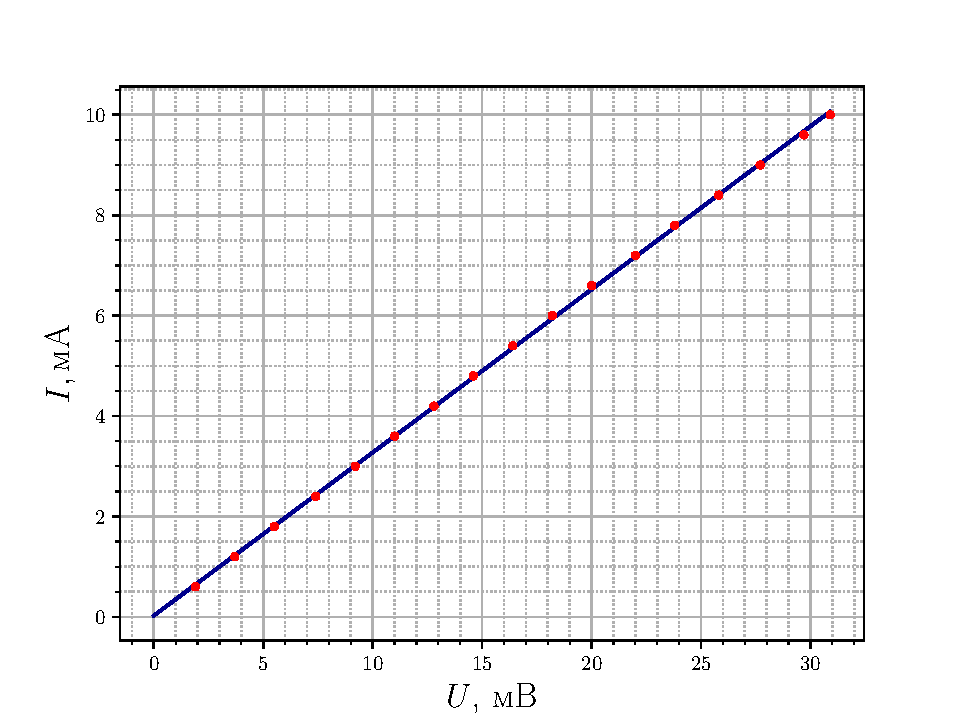
\includegraphics[width=\linewidth]{fig/52.pdf}
	\caption{Вольт-амперная характеристика образца}
	\label{fig:5.2}
\end{minipage}
\hfill
\begin{minipage}[h]{0.49\linewidth}
	\centering
	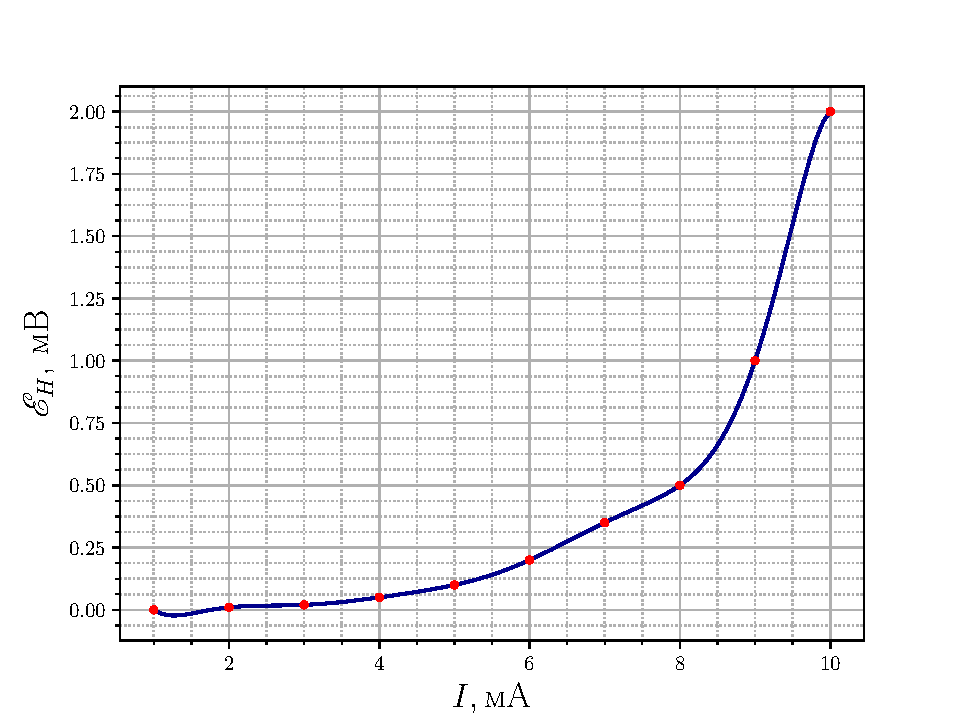
\includegraphics[width=\linewidth]{fig/53.pdf}
	\caption{Зависимость паразитного напряжения на образце от тока образца}
	\label{fig:5.3}
\end{minipage}
\end{figure}



На рис. \ref{fig:5.3} изображена зависимость паразитного напряжения на образце от тока образца. Она понадобится нам при вычислении коэффициента Холла. 




\subsection{Определение типа основных носителей в образце}

\begin{figure}[h!]
	\centering
	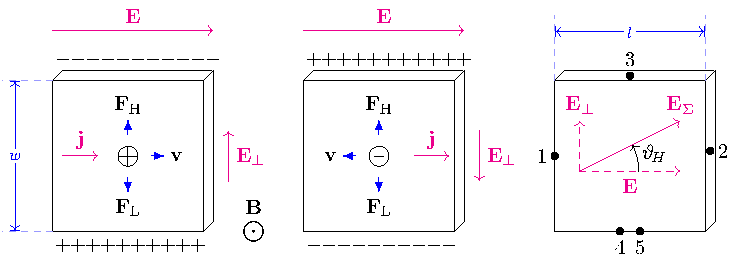
\includegraphics[width=0.7\linewidth]{fig/effect.pdf}
	\caption{Смещение носителей заряда соответственно в дырочном и электронном полупроводниках}
	\label{fig:hall}
\end{figure}

\subsection{Расчёт постоянной Холла и подвижности основных носителей}
Согласно формуле \eqref{eq:2.5}, зная величину тока или магнитного поля , можно найти\footnote{Приводить расчёты я, конечно же, не буду. Если хочется их увидеть, то они произведены в скриптах  или в самом \TeX-файле на моем Github'e. Очень надеюсь, ошибок в порядках} из рис.\ref{fig:5.5}-\ref{fig:5.6} отношение постоянной Холла к его поперечному размеру.


Из рис. \ref{fig:5.5} для четырех значений тока (индексы соответствуют значению тока):
\begin{itemize}
	\item $R_1= \frexp{R1} \Rdim$
	\item $R_2= \frexp{R2} \Rdim$
	\item $R_4= \frexp{R4} \Rdim$
	\item $R_7= \frexp{R7} \Rdim$ (Здесь не учтен паразит).
\end{itemize}


Чтобы точнее вычислить отношение $\frac{\E}{I}$ в  рис. \ref{fig:5.6} учитывалось паразитное напряжение, найденное выше: экспериментальные данные аппроксимировались методом наименьших квадратов с учетом веса каждой точки. Для четырех значений магнитного поля (индексы соответствуют значению магнитного поля в Гс):
\begin{itemize}
	\item $R_{200}= \frexp{R200} \Rdim$ 
	\item $R_{400}= \frexp{R400} \Rdim$
	\item $R_{600}= \frexp{R600} \Rdim$
	\item $R_{900}= \frexp{R900} \Rdim$
\end{itemize}

Посчитав значение постоянной Холла и удельной проводимости, можем оценить подвижность основных носителей в образце:
\begin{equation}
	\mu_H= R\cdot \sigma
\end{equation}
Усредненная по восьми значениям коэффициента Холла величина подвижности:

\begin{equation}
	\mean{\mu_H}=\frexp{mu} \frac{\text{м}^2}{\text{В}\cdot \text{c}}
\end{equation}
%% ВНИМАНИЕ!!! На самом деле в этом опыте значение R получилось в 100 раз больше. Стоит разобраться почему так
А из формулы \eqref{eq:2.7} можем оценить концентрацию носителей:

\begin{equation}
	\mean{n} = \frexp{n} \frac{1}{\text{м}^3}
\end{equation}

% section  (end)
\begin{figure}[H]
	\centering
	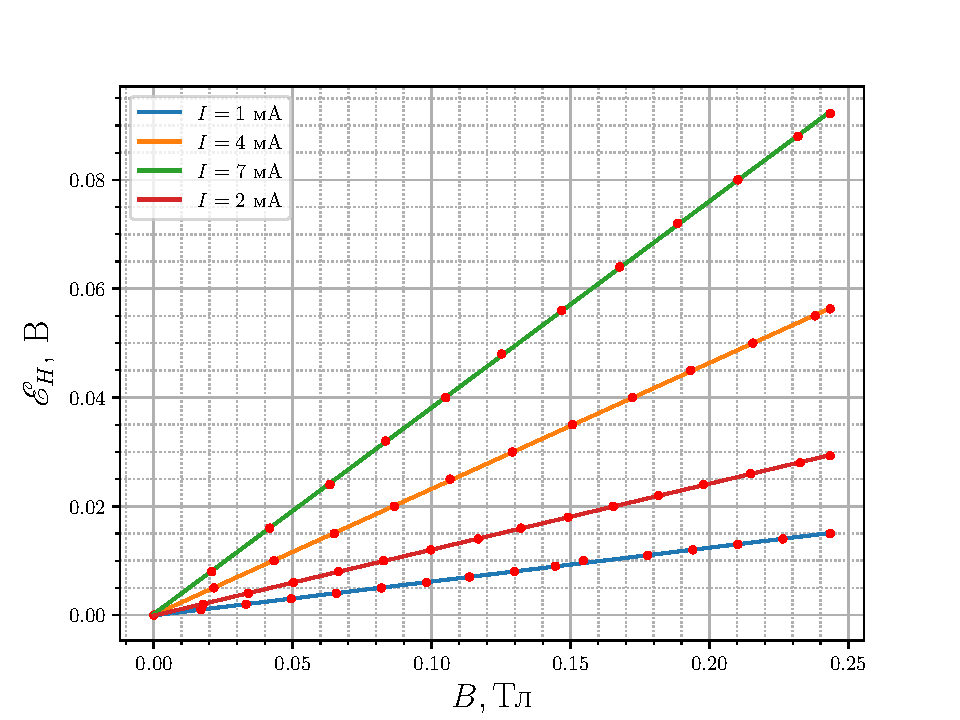
\includegraphics[width=\linewidth]{fig/55.pdf}
	\caption{Зависимость ЭДС Холла от магнитного поля при нескольких фиксированных значениях тока образца.}
	\label{fig:5.5}
\end{figure}

\begin{figure}[H]
	\centering
	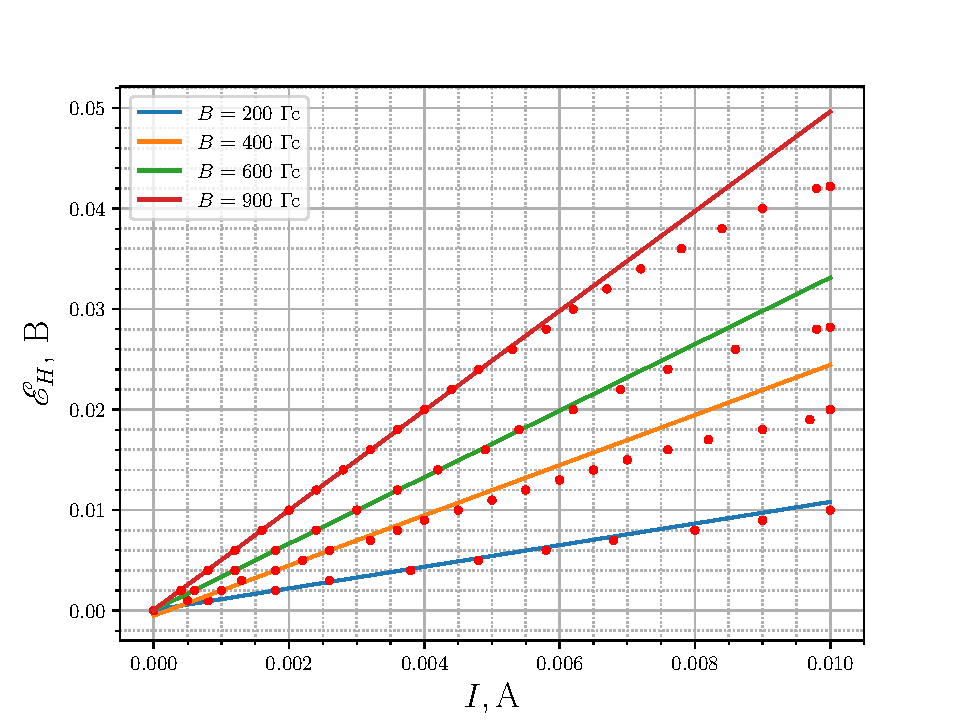
\includegraphics[width=\linewidth]{fig/56.pdf}
	\caption{Зависимость ЭДС Холла от тока образца при нескольких фиксированных значениях магнитного поля.}
	\label{fig:5.6}
\end{figure}
\section{Заключение}
В данной работе был изучен эффект Холла, определен тип носителей заряда исходного образца, а также определены следующие величины:
\begin{itemize}
	\pyc{R=mean(R)}
	\item $\mean{R}=\frexp{R} \,\Rdim $
	\item $\mean{n}=\frexp{n} \,\frac{1}{\text{м}^3}$
	\item  $\mean{\mu_H}=\frexp{mu}\, \frac{\text{м}^2}{\text{В}\cdot \text{c}}$
	\item $\sigma=\frexp{sigma}\, \frac{\text{м}}{\text{Ом}}$,
\end{itemize}
где $\mean{R}$ - среднее значение постоянной Холла, $\mean{n}$ - среднее значение концентрации основных носителей, $\sigma$ - удельная проводимость образца, $\mean{\mu}$ - среднее значение подвижности основных носителей.


\begin{thebibliography}{}
	\bibitem{lit0} Сарафанов Ф.Г. Блог <<\href{http://fedorsarafanov.github.io}{Physics \& other}>>. Н.Новгород: РФФ ННГУ, 2019.
	\bibitem{lit1} Киттель Ч. Введение в физику твердого тела. М.: Наука, 1978.
	\bibitem{lit2} Мермин Н. Физика твердого тела. Том 1,2. М.: Мир, 1979.
	\bibitem{lit3} Битюрин Ю.А. и др. Измерение ширины запрещенной зоны. Описание к лабораторной работе. Н.Новгород: ННГУ, 2004
	\bibitem{lit4} Воробьев Л.Е. Механизмы рассеяния носителей заряда в полупроводниках: учебное пособие. Ленинград: ЛПИ, 1988.
	\bibitem{lit5} Зи С.М. Физика полупроводниковых приборов. М.: Сов. Радио, 1984.
	\bibitem{lit6} Пожела. Ю. Физика быстродействующих транзисторов. Вильнюс: Мокслас, 1989.
	\bibitem{lit7} Бонч-Бруевич В.Л. Калашников С.Г. Физика полупроводников. М.: Наука, 1990.
	\bibitem{lit8} Орешкин П.Т. Физика полупроводников и диэлектриков. М.: Высшая школа, 1976.
	\bibitem{lit9} Кучис Е.В. Методы исследования эффекта Холла. М.: Сов. Радио, 1974.
\end{thebibliography}


\end{document}